\documentclass[10pt]{article}
\usepackage[utf8]{inputenc}
\usepackage[myheadings]{fullpage}
\DeclareUnicodeCharacter{0301}{\hspace{-1ex}\'{ }}

% Package for headers 
\usepackage{fancyhdr}
\usepackage{lastpage}
\usepackage{pdfpages}

% For figures and stuff
\usepackage{graphicx, wrapfig, subcaption, setspace, booktabs}
\usepackage[T1]{fontenc}

% For lists
\usepackage{enumitem}
\usepackage{booktabs}

% Change for different font sizes and families
\usepackage[font=small, labelfont=bf]{caption}
\usepackage{fourier}
\usepackage[protrusion=true, expansion=true]{microtype}
\usepackage{url}

% Maths
\usepackage{amsmath,amssymb}
\usepackage{float}
\usepackage{graphicx}
\usepackage{wrapfig}
\usepackage[colorinlistoftodos]{todonotes}
\usepackage[colorlinks=true, allcolors=blue]{hyperref}

% For python code
\usepackage{color} 
\usepackage{listings} 
\usepackage{setspace} 

\definecolor{Code}{rgb}{0,0,0} 
\definecolor{Decorators}{rgb}{0.5,0.5,0.5} 
\definecolor{Numbers}{rgb}{0.5,0,0} 
\definecolor{MatchingBrackets}{rgb}{0.25,0.5,0.5} 
\definecolor{Keywords}{rgb}{0,0,1} 
\definecolor{self}{rgb}{0,0,0} 
\definecolor{Strings}{rgb}{0,0.63,0} 
\definecolor{Comments}{rgb}{0,0.63,1} 
\definecolor{Backquotes}{rgb}{0,0,0} 
\definecolor{Classname}{rgb}{0,0,0} 
\definecolor{FunctionName}{rgb}{0,0,0} 
\definecolor{Operators}{rgb}{0,0,0} 
\definecolor{Background}{rgb}{0.98,0.98,0.98} 
 
\lstdefinelanguage{Python}{ 
  numbers=left, 
  numberstyle=\footnotesize, 
  numbersep=1em, 
  xleftmargin=1em, 
  framextopmargin=2em, 
  framexbottommargin=2em, 
  showspaces=false, 
  showtabs=false, 
  showstringspaces=false, 
  frame=l, 
  tabsize=4,
  % Basic 
  basicstyle=\ttfamily\small\setstretch{1}, 
  backgroundcolor=\color{Background}, 
  % Comments 
  commentstyle=\color{Comments}\slshape, 
  % Strings 
  stringstyle=\color{Strings}, 
  morecomment=[s][\color{Strings}]{"""}{"""}, 
  morecomment=[s][\color{Strings}]{'''}{'''}, 
  % keywords 
  morekeywords={import,from,class,def,for,while,if,is,in,elif,else,not,and,or,print,break,continue,return,True,False,None,access,as,,del,except,exec,finally,global,import,lambda,pass,print,raise,try,assert}, 
  keywordstyle={\color{Keywords}\bfseries}, 
  % additional keywords 
  morekeywords={[2]@invariant,pylab,numpy,np,scipy}, 
  keywordstyle={[2]\color{Decorators}\slshape}, 
  emph={self}, 
  emphstyle={\color{self}\slshape}, 
  % 
} 
 
\linespread{1.3}


% Bibliography
\usepackage[style=ieee, refsection=chapter, backref=true]{biblatex}
\usepackage{csquotes}
\usepackage{multicols}
\usepackage{wrapfig}
\addbibresource{references.bib}

%% Language and font encodings
\usepackage[english]{babel}
\usepackage{csquotes}
\usepackage{todonotes}


\newcommand{\HRule}[1]{\rule{\linewidth}{#1}}
\onehalfspacing
\setcounter{tocdepth}{5}
\setcounter{secnumdepth}{5}

%% Sets page size and margins
\usepackage[a4paper,top=2cm,bottom=1.5cm,left=2cm,right=2cm,marginparwidth=1.5cm]{geometry}

\pagestyle{fancy}
\fancyhf{}

% Header and footer information
\setlength\headheight{15pt}
% \fancyhead[L]{s1000000} 
\fancyhead[R]{B. Klein Ikkink}
\fancyfoot[R]{\thepage}
\setlength {\marginparwidth }{2cm}

\begin{document}

\date{}

% Do not change anything here except in \LARGE \textbf{This is the title of the essay} 
% /hline before and after the title makes those horoziontal lines appear, you can change the appearance by changing the 2pt to different sizees
\title{ \normalsize Engineering Physics, The Hague University of Applied Sciences, Delft
		\\ [1.0cm]
		% Change to your faculty if needed
		
\includegraphics[width=100mm]{img/misc/hhs_en_groen_hex.png}  %\\[.5cm]
		%and   \\[.5cm]
		%\includegraphics[width=50mm]{img/company_Logo.png}\\[.5cm]
		%\normalsize Company Name \\ [1.0cm]
		%Faculty of Social Sciences\\
		\HRule{2pt} \\
		\LARGE \textbf{Development custom instrumentation for the Remote-controlled fabrication of 2D heterostructuren} %para que quede encerrado en las lineas
		\HRule{2pt} \\ [0.5cm]
		\normalsize \today \vspace*{5\baselineskip}}
		
\date{}

\author{
        Report by:\\
		B. Klein Ikkink            \\[1cm]
		 Supervised by:        \\
		 S. Bhattacharyya, LION \\
		 F. Galli, LION \\
		 }
		 
\maketitle
\pagenumbering{roman}

\clearpage
\section*{Foreword}
First of all I would like to thank my internship supervisors Dr. S. Bhattacharyya \& Dr. F. Galli for taking the chance and giving me the freedom to do this project without much guidance and in my own way.
I learned more than I could have imagined and got a clear picture of what I want to do with my future, I am just starting.
I Also want to thank both for giving me the chance to release the project under open source license, so it will be possible for others to recreate the instrument without licensing extra cost.\\

Furthermore I would like to thank R. Stoelwinder from LU FMD and P. Nimberi from LU ELD (Leiden University Electronics Department) for the invaluable lessons I learned about product development and the field of fine mechanics and electronics.
You both helped me raise the project to a higher standard and without both of you the performance wouldn't have been anywhere near where it is today.

\todo{Finish the foreword}
\todo{also thank M. Hesselbert for the help with the positioning of the stages}

\clearpage

\section*{Abstract}
\todo{Create the abstract}
\clearpage

\newpage

\tableofcontents
\newpage

\section*{Used abbreviations}
\label{ap:veel_gebruikte_symbolen}
\todo{pagina nummering pas hier beginnen, voorgaande in romeinse nummering}
\begin{itemize}[noitemsep]
    \item LION : Leiden Institute Of Physics
    \item LU: Leiden University
    \item VDWSF: Van Der Waals Stacking Facility
    \item FMD : Fine Mechanical Department
    \item ELD : Electronics Department
    \item CLI : Command Line Interface
    \item GUI : Graphical User Interface
    \item SDK : Software Development Kit
    \item DAS : Domain Applied Science

\end{itemize}

\clearpage
\pagenumbering{arabic}

\section{Introduction}
\todo{Rephrase the text so it isn't flagged as plagiaat}
The discovery of graphene in 2004, awarded the Nobel Prize in Physics in 2010, has led to a completely new field of research based on 'atomically thin materials', materials of a few atomic layers thick (2D materials). 
Recently, the focus of the research area has shifted to fabricating completely new structures by stacking different atomically thin materials 'Van Der Waals Heterostructures'. 
Atomic thin materials can consist of metals, semiconductors, insulators, ferromagnets, superconductors, etc., combining these materials is a route to developing useful devices \cite{geimVanWaalsHeterostructures2013}.
Although there has been research done on the efficient and accurate fabrication of van der Waals Heterostructures and several groups have released papers about these methods and instuments, the literature is lacking of comprehensive technical papers providing enough detail for reproducing such systems by other groups \cite{gantSystemDeterministicTransfer2020,castellanos-gomezDeterministicTransferTwodimensional2014}.\\

Recently, a new research group was started under Principle Investigator Dr. Semonti Bhattacharyya who is an expert in fabricating and characterizing Van Der Waals Heterostructures and 2D materials and who recently started her new laboratory at LION, the Van Der Waals Stacking Facility (VDWSF).
This project will focus on the efficient and accurate fabrication and imaging of the Van Der Waals Heterostructures.
One of the side goals of the project is also to contribute to the avalailable literature on reproducing stacking setups for the fabrication of van der Waals Heterostructures.
LION is one of the oldest physics research institutes in the Netherlands. 
The research performed at Leiden Institute of Physics covers a broad spectrum of topics, from cosmology to condensed matter physics, from quantum computers to new systems such as Van Der Waals Heterostacks.
Research at LION is largely fundamental and curiosity-driven but also with an eye toward societal value. \\

\todo{Add some text about the importance of releasing the paper open source so it can be used as a starting template}


\clearpage
\section{Project definition}
\noindent Presently a commercial setup \cite{HQGrapheneSystemsDesigns} for fabricating 2D Hetero-stacks is used in the Van Der Waals Stacking Facility (VDWSF) laboratory at LION. 
This commercial setup is prone to vibrations and has an inferior-quality microscope, which makes it difficult to clearly identify small 2D material.
Furthermore, the laboratory has a vibration level slightly above VC-C \cite{isolationVibrationCriterionVC} \ref{ap:GEOPhone_measurement}.
For these reasons in combinations with the scarcity in papers on the reproducing existing setups \cite{gantSystemDeterministicTransfer2020,castellanos-gomezVanWaalsHeterostructures2022} a new setup will be developed that is less sensitive to mechanical vibrations.
The setup is focused on improved rigidity, accuracy and flexibility compared to the commercially available and previous versions.
The setup will be based on a commercial (Olympus BXFM) optical microscope, but to reach the goal a custom microscope stand, sample holder, mask holder and software have to be developed.

\subsection{Research question}
\begin{center}
    \textit{What components and control techniques should be used to make the stacking setup as least susceptible to vibration as possible and controllable at the sub-micrometer scale while producing clear images with an optical microscope?}
\end{center}

\subsection{Research goal}
\begin{center}
    \textit{Building a stacking setup that is as least susceptible to vibration as possible where the base x-y-z stages move with resolution on the micrometer scale and the mask x-y-z stages on the nanometer scale, which can be remotely controlled, while being able to capture clear images with an optical microscope and is modifiable/upgradable by the end user.}
\end{center}

\clearpage
\section{Background}


\begin{figure}[H]
  \centering
  \begin{minipage}[b]{0.58\textwidth}
    \includegraphics[width=\textwidth]{img/misc/Flake388.png}
    \caption{Image of an MOS2 flake acquired using an optical microscope, The flake was exfoliated using the scotch-tape method. By J. Scheffer}
    \label{fig:MOS2_flake_joost}
  \end{minipage}
  \hfill
  \begin{minipage}[b]{0.38\textwidth}
    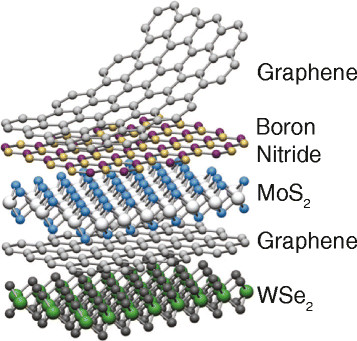
\includegraphics[width=\textwidth]{img/misc/vdws_example.png}
    \caption{Simplified schematic of the principle of van der Waals Heterostructures. By stacking different 2D material flakes in a specific order nano devices with useful properties \cite{jungSurfaceEffectsElectronic2014, geimVanWaalsHeterostructures2013}.}
    \label{fig:heterostack_schematic}
  \end{minipage}
\end{figure}

Over the past decade, research into two-dimensional (2D) materials and van der Waals heterostructures has opened up a world of possibilities for the development of new technologies. 2D materials, such as graphene and hexagonal boron nitride, are atomically thin crystalline structures and have unique electrical, optical, and mechanical properties that make them interesting for a wide variety of applications.
Van der Waals Heterostructures are nano-devices composed of two or more 2D material flakes like the flake shown in figure \ref{fig:MOS2_flake_joost} that are stacked together and can be used to create electronic and optoelectronic nano devices as shown in figure \ref{fig:heterostack_schematic}.
This research has enabled the development of a wide range of technologies, including flexible electronics, high-speed transistors, and ultra-sensitive sensors. 
The promise of 2D materials and van der Waals heterostructures is that they can be used to create devices that are faster, more efficient, and more reliable than existing technologies \cite{geimVanWaalsHeterostructures2013}.

\subsection{Fabrication of van der Waals Heterostructures}
Due to the fact that the area of 2D materials and van der Waals Heterostructures is relatively new there are various ways of fabricating these structures, each with their own drawbacks.
Some of the most used methods are: PMMA carrier method, PDMS dry transfer and the van der Waals pick-up method
For this project the van der Waals pick-up method is used as this method has no need for wet chemicals and yields the cleanest samples relative to the other methods as only the top most layer of the heterostructures makes contact with a polymer, this is an important factor to consider as contamination on the interface between layers can affect the properties of the created heterostructures \cite{pizzoccheroHotPickupTechnique2016,frisendaRecentProgressAssembly2018}.\\

There are small variations in the protocols found in the literature but the general van der Waals pick-up method is as follows:
\todo{ref naar variaties in literatuur invoegen}
\begin{enumerate}[noitemsep]
\item A substrate with exfoliated flakes is prepared an placed on the working surface of the instrument
\item The flake that has to form the top of the heterostack is exfoliated onto a layer of PDMS film (the stamp) and placed on a micromanipulator for alignment.
\item The stamp is lowered onto the target flake until the stamp flake makes contact with the target flake.
\item As both of the flakes are atomically flat, the contact area and thus the adhesion due to the van der Waals force between the flakes can be very large.
By slowly lifting the stamp the flake can be picked up from the substrate.
\item By repeating the process with new flakes on the substrate a stack of multiple layers of different 2D material flakes can be created.
\item When the stack contains the wanted layers the stack can be released by making contact with a clean substrate and heating the PDMS to $110^\circ$C.
Temperatures above $110^circ$C favour van der Waals adhesion between the flakes over the adhesion between the PDMS and the top flake, resulting in a release of the stack from the PDMS \cite{pizzoccheroHotPickupTechnique2016}.
\end{enumerate}

 This process consists of serval time consuming steps, such as finding suitable flakes, placing the flakes on the stamp and substrate, and changing the sample temperature.


\subsection{Monash University setup}

\begin{figure}[H]
  \centering
  \begin{minipage}[b]{0.45\textwidth}
    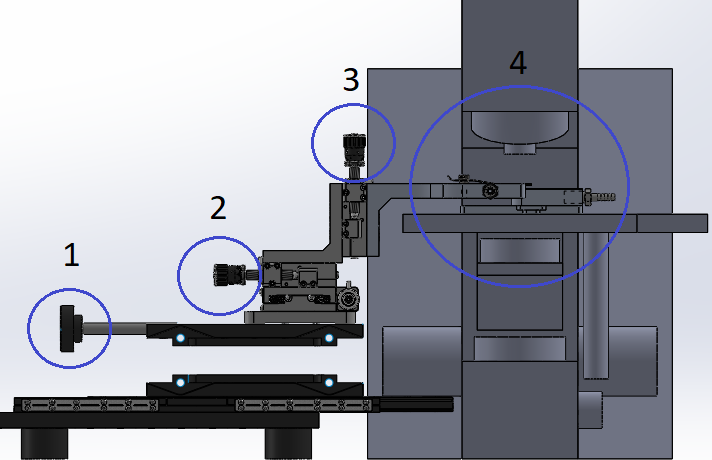
\includegraphics[width=\textwidth]{img/design_cycle/monash_frond_view_with_markings.png}
    \caption{Frond view of the Monash University stacking setup design. Where \textbf{(1)} is the course mask z-stage actuator, \textbf{(2)} the mask x and y actuator (the y actuator is not visible in this image but is positioned on a 90degree angle with the x-stage actuator), \textbf{(3)} the fine mask z-stage actuator and \textbf{(4)} the workspace of the setup.}
    \label{fig:monash_frond}
  \end{minipage}
  \hfill
  \begin{minipage}[b]{0.53\textwidth}
    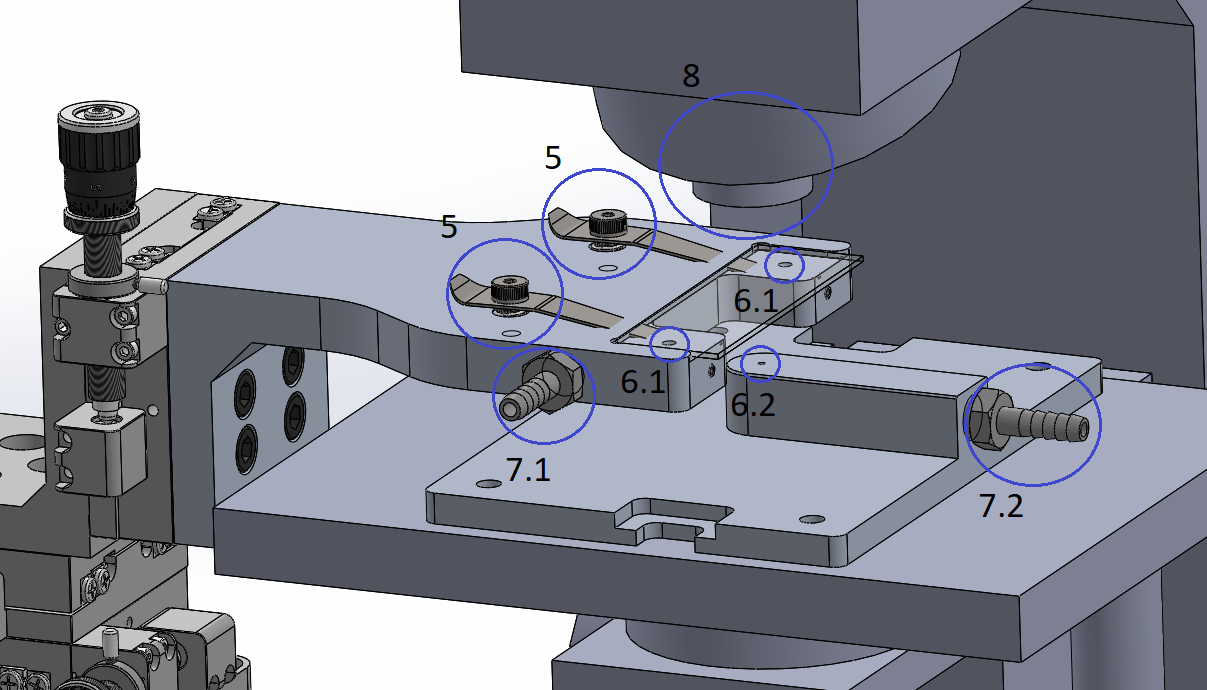
\includegraphics[width=\textwidth]{img/design_cycle/monash_workspace_with_markings.png}
    \caption{Zoomed in view of the workspace in the Monash University stacking setup. Where \textbf{(5)} are the clamps used to keep the glass slide with the stamp on it in place, \textbf{(6)} vacuum holes used for additional clamping force if needed. Due to the clamps for the mask holder the vacuum holes in the mask (6.1 and 6.2) might seem redundant, and for additional clamping force, they are. The vacuum holes in the mask are used for phase correction between the mask and sample-holder for the introduces vibration due to the vacuum pump. \textbf{(7)} are the connections for the vacuum tubes, \textbf{(8)} the used objectives of the microscope.}
    \label{fig:monash_side}
  \end{minipage}
\end{figure}

As inspiration for the base design the stacking setup from Monash University was used (see figure \ref{fig:monash_frond} and \ref{fig:monash_side}), for which the models were provided by Dr. S. Bhattacharyya. 
The Monash University setup is an example of a general design used for stamping instruments in atmosphere and in isolated environments \cite{castellanos-gomezDeterministicTransferTwodimensional2014,zhaoInexpensiveSystemDeterministic2020,gantSystemDeterministicTransfer2020}
While the designs of Monash setup is not optimal it is well suited to use as a precursor for the follow up designs. 
The Monash setup contains most of the functionality that are needed for the stamping procedure, such as sample heating and cooling, mask x-y-z-manipulation (1, 2, and 3 in figure \ref{fig:monash_frond}) and the option to use a low powered vacuum to keep the sample in place (6 and 7 in figure \ref{fig:monash_side}).
While the parts fulfill their purpose, there is room for improvement, mostly in the reduction of redundant materials and the reordering of the components to reduce cantilevers in the setup.
For practical purposes extra degrees of freedom can be added to give the end-user more freedom in manipulating the instrument.

\subsection{Criteria}
\label{ch:criteria}
\todo{insert reference to monash and hqgraphene setup}
By analyzing the workflow of the manual and motorized commercial stamping setups \cite{castellanos-gomezDeterministicTransferTwodimensional2014,gantSystemDeterministicTransfer2020,huangReliableExfoliationLargeArea2015,HQGrapheneSystemsDesigns,zhaoInexpensiveSystemDeterministic2020} two different functional decompositions were made, ( see appendix \ref{ap:hardware_functional_decomposition} and \ref{ap:software_functional_decomposition}). Using these decompositions and the workflow analysis a set of criteria the instrument should follow was made.

\begin{enumerate}[noitemsep]
  \item Mask holder
  \begin{enumerate}[noitemsep]
    \item The mask should be motorized and able to move in the x, y and z direction with a resolution of $>30$ nm.
    \item The pitch of the mask should be able to be adjusted with a resolution of $>0.05^{\circ}$.
    \item The yaw of the mask should be able to be adjusted with a resolution of $>0.05^{\circ}$, with a minimum range of $180^{\circ}$.
  \end{enumerate}
  \item Sample holder
  \begin{enumerate}[noitemsep]
    \item The sample holder should be able to hold a minimum of 2 samples.
    \item The sample should be able to heat with a ramp speed of $2.0 - 50.0^{\circ} C/s$
    \item The sample should be able to cool with a ramp speed of $-0.1 - 30.0^{\circ} C/s$ 
    \item The sample holder should be able to operate between $20^\circ$C and $220^\circ$C
  \end{enumerate}
  \item Microscope \& stand
  \begin{enumerate}[noitemsep]
    \item Due to the fact that the VDWSF laboratory has problems with external vibrations (see appendix \ref{ap:vibrational_measurement}) the microscope stand should be as rigid as possible to make the instrument behave like one rigid body instead of a system of multiple dampened bodies.
    \item The microscope should a 20x objective with correction collar to be able to focus on the sample through the mask holder glass slide.
  \end{enumerate}


\end{enumerate}

\subsection{Vibration isolation}
\label{ch:vibration_isolation}
During the design phase of the project it is important to take the susceptibility to vibration of the instrument into account due to the fact that the VDWSF lab has vibrational issues when no dampeners are used as seen in appendix \ref{ap:vibrational_measurement}.
With commercial stacking setups external vibrations are a known issue during the stacking process. 
Due to instrument not vibrating in phase, the phase difference between the mask and the sample can cause tearing in the flake, positioning the flake also becomes more cumbersome.
With higher amplitude vibrations focussing the microscope also becomes an issue.
Because no commercial product complied with the set criteria, the microscope stand is developed in house in collaboration with LU FMD (Leiden University Fine Mechanical Department).\\

When studying the response of an instrument to external vibration the choice between modelling force or amplitude driven vibrations has to be made.
Intuitively these might seem similar but the mathematics to describe the system differ significantly \cite{hesselberthMicroscopieBeweging}.
Due to the the situation the instrument will be placed in (non dampened optical table) the amplitude driven model was chosen as amplitude driven vibration will have the dominant effect in the system (force driven vibrations can only be exerted by the atmosphere surrounding the instrument and are neglected).

\begin{figure}[H]
  \centering
  \begin{minipage}[b]{0.30\textwidth}
    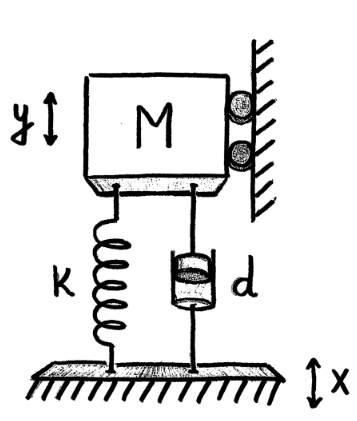
\includegraphics[width=\textwidth]{img/resonance/simplified_1DOF_oscilator.png}
    \caption{Schematic of a simplified microscope as a mass spring dampener system on a vibrating base. \cite{hesselberthMicroscopieBeweging}}
    \label{fig:1DOFoscilator}
  \end{minipage}
  \hfill
  \begin{minipage}[b]{0.65\textwidth}
    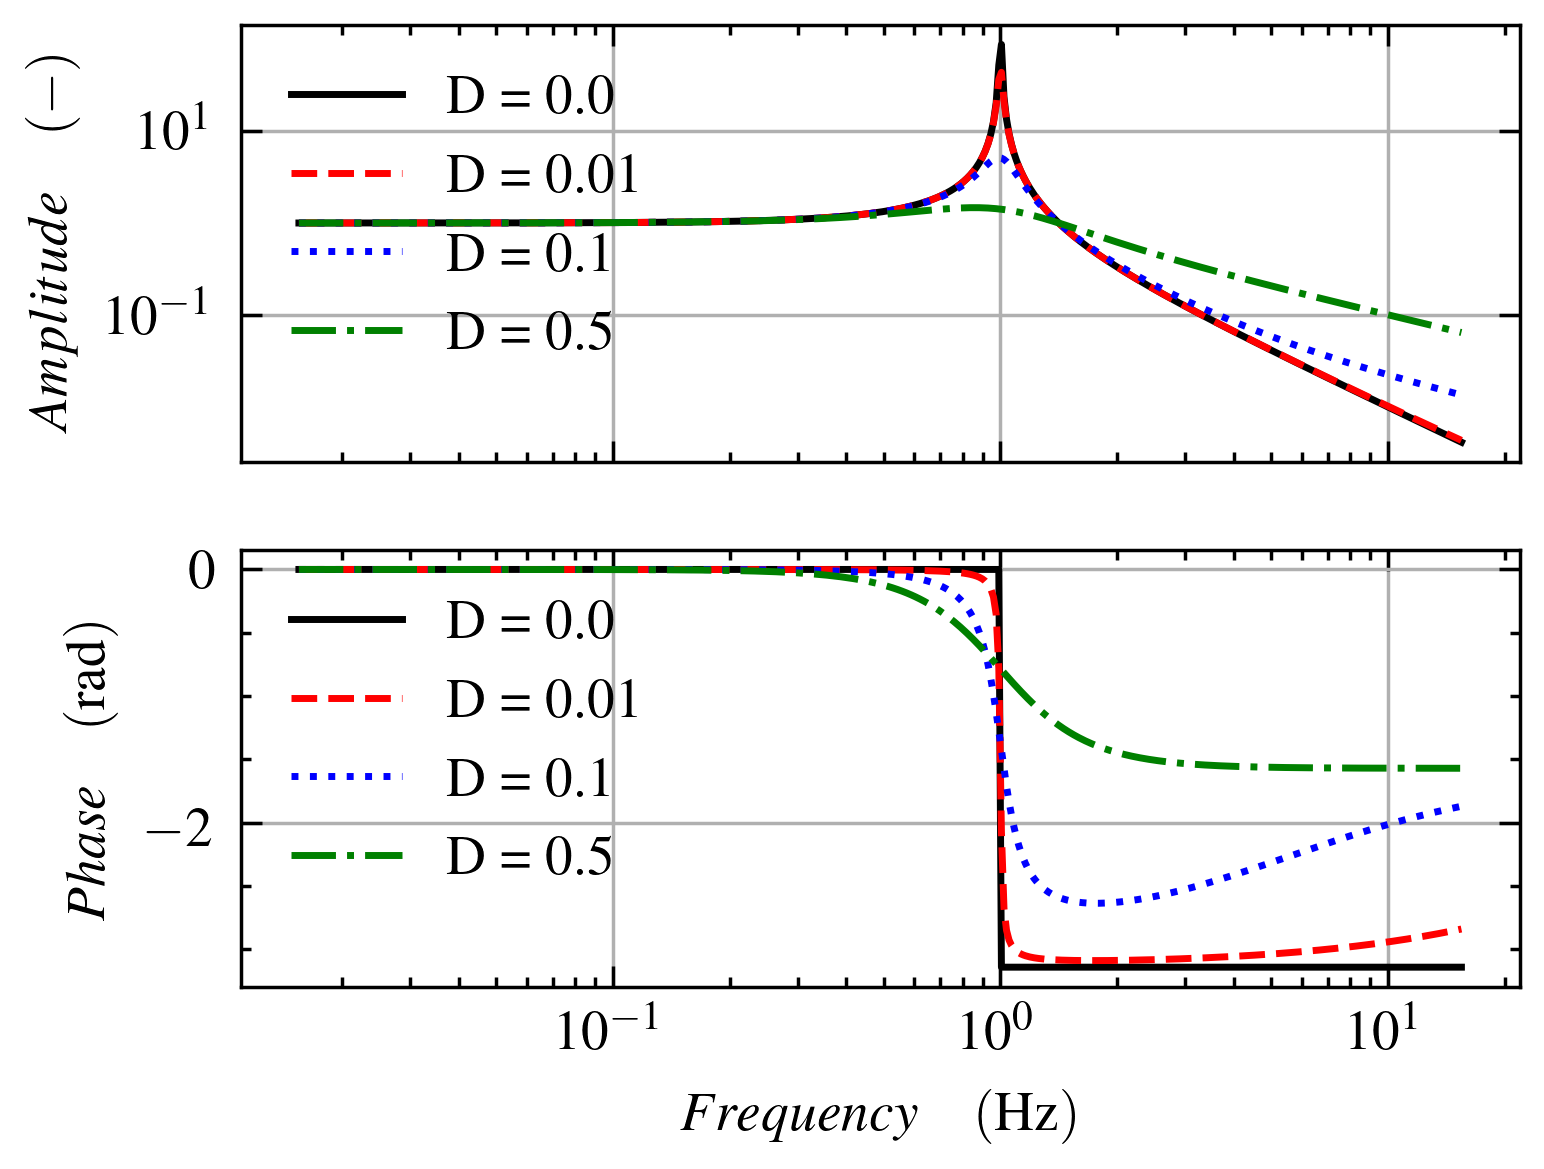
\includegraphics[width=\textwidth]{img/resonance/1dof_oscillator_without_damping.png}
    \caption{Amplitude (top) and phase (bottom) as a function of frequency according to equation \ref{eq:bode_amplitude}}
    \label{fig:amp_driven_bode}
  \end{minipage}
\end{figure}

The amplitude driven model consists of a simplified mass spring system, where the microscope head represents the mass and the stand the spring as seen in figure \ref{fig:1DOFoscilator}.
By representing the system a such control theory can be used to approximate the dynamic behavior of the instrument. 
To simplify calculations the system is separated in two separate inertial systems.
System $Y$ with amplitude $y$ to represent the defection of the microscope head with mass $m$ from the equilibrium position and system $X$ with amplitude $x$ to represent the defection of the base with respect to the equilibrium position.
From these two inertial systems the force balance given in equation \ref{eq:krachten balans instrument} can be derived.\\
 
Because the response as a function of time is not of interest for this system the transfer function of the system can be studied in the Laplace space, reducing the complexity of the needed calculations.
The transfer function derived from the force balance (equation \ref{eq:krachten balans instrument}) is given in equation \ref{eq:trilling overdracht met demping}.
By substituting the equations given in equation \ref{eq:transfer_substitutions} in to equation \ref{eq:trilling overdracht met demping} the number of dimensions in the equation can be reduced from four to two and it becomes possible to study the generalized behavior.
Equation \ref{eq:trilling overdracht met demping} can also be used to model the response of a system with a given mass and hooke constant, but due to the complex geometric shape of the instrument the general model was chosen.

\begin{equation}
    m \frac{\mathrm{d}^2 y}{\mathrm{d} t^2} + d \frac{\mathrm{d}y}{\mathrm{d}t} +ky = d\frac{\mathrm{d}x}{\mathrm{d}t} + kx
    \label{eq:krachten balans instrument}
\end{equation}

\begin{equation}
    \omega_0 = \sqrt{\frac{k}{m}}; \quad D = \frac{d}{\sqrt{2mk}}; \quad f = \frac{\omega}{\omega_0}\rightarrow \omega = f\omega_0
    \label{eq:transfer_substitutions}
\end{equation}

\begin{equation*}
    H = \frac{Y}{X} = \frac{dj\omega + k}{-m\omega^2 +dj\omega + k} = \frac{\omega_0^2 +2jD \omega_0 \omega}{\omega_0 + 2jD\omega_0 \omega - \omega} = \frac{1 + 2jDf}{1+ 2jDf - f^2}
    \label{eq:trilling overdracht met demping}
\end{equation*}

\begin{equation}
    H = \frac{1 + 2jDf}{1+ 2jDf - f^2} = \frac{1}{1 - f^2}\quad \mathrm{v}\quad D = 0
    \label{eq:trilling overdracht zonder demping}
\end{equation}

\begin{equation}
    A = \frac{1}{(1-f^2)^2}; \quad \phi = \arctan{\left( \frac{0}{1 - f^2}\right)}
    \label{eq:bode_amplitude}
\end{equation}

The Bode plot of the transfer function is given in figure \ref{fig:amp_driven_bode}.
As expected the system has a peak amplitude at the resonance frequency, but the phase shows an unexpected result when compared to the expected force driven behavior.
The phase of the system wil shift with $\pi$ when a frequency above the eigen-frequency of the system is reached, this means that for all frequencies (including the eigen-frequency) the system will vibrate in phase.
This solves the problem of the out of phase vibrations but also introduces the new problem of the undamped resonance peak at the eigen-frequency of the system.

\begin{equation}
  W = ma \int_{A_0}^{A_n} \mathrm{d}A = maA \rightarrow A \propto \frac{1}{m}
  \label{eq:wave_energy}
\end{equation}

As shown in equation \ref{eq:wave_energy} the work needed to get the instrument in motion is proportional to the mass of the instrument.
This means that by increasing the mass of the system the energy needed to get it in motion can be raised to such a level that it is realistically not possible to get the instrument in motion by amplitude driven vibrations alone.
A tradeoff of this solution is that the eigen-frequency given by equation \ref{eq:transfer_substitutions} will shift down, this can cause problems when combined with the low frequencies present in the VDWSF lab (see appendix \ref{ap:vibrational_measurement}).\\

%Het instrument zelf zal geen demping hebben maar geplaats worden op een actieve vibratie isolatie tafel, voor correcte werking is het van belang dat de resonantiefrequenie van het instrument buiten de doorgelaten band van de actieve tafel valt. Voor de gebruikte active demper is dit 90\% vanaf $2$ Hz en 99\% vanaf $10$ Hz \cite{DVIATTabletopActive}
%\todo{Aantonen dat een hoge dichtheid (en dus massa) de resonantie frequentie verhogen}

%\begin{figure}[htp]
%  \centering
%  \begin{minipage}[b]{0.49\textwidth}
%    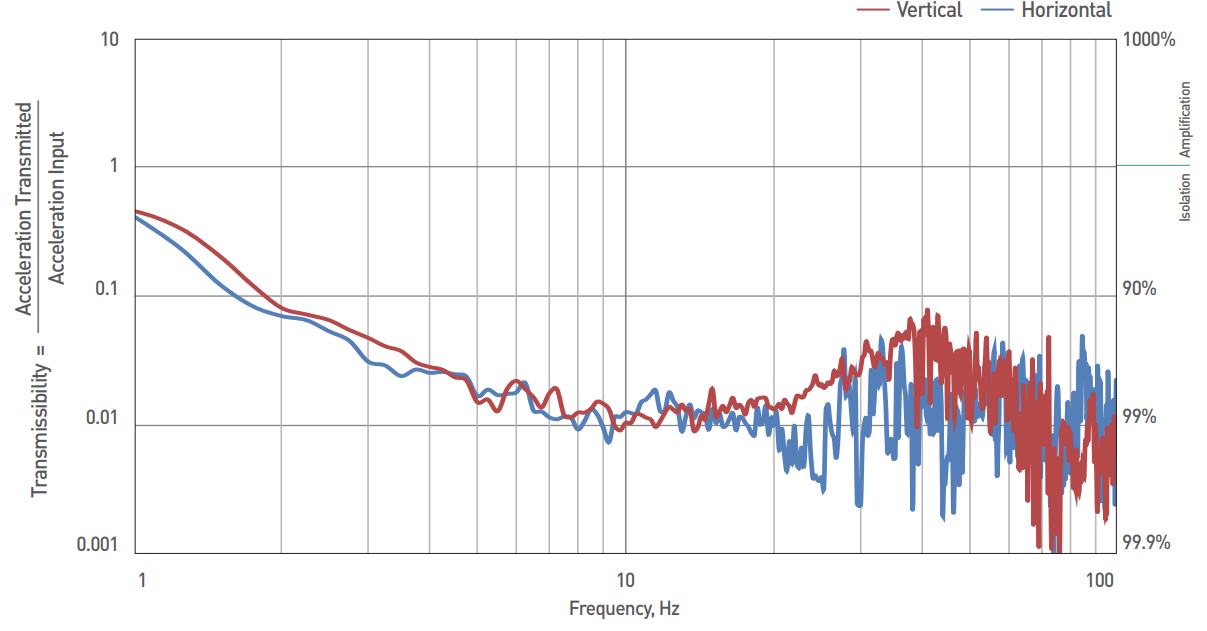
\includegraphics[width=\textwidth]{img/resonance/damping_table_response.png}
%    \caption{}
%    \label{fig:damp_table_response}
%  \end{minipage}
%\end{figure}

\todo{uitzoeken aan welke vc norm wij willen voldoen}
\todo{betekenis van NIST-A norm uitzoeken}

\section{Methods \& Results}
In the next chapters the methods and results used for the development of the instrument are discussed.

\subsection{Stand design}
One of the main issues in the stamping process is the susceptibility to vibrations caused by external factors as described in \ref{ch:vibration_isolation}.
The VDWSF only complies to VC-A (see appendix \ref{ap:vibrational_measurement}), this means the external vibrations have to be taken into account when designing the instrument, especially the stand of the microscope. 
Due to the fine mechanical nature of the design and fabrication of the microscope stand the process was done in collaboration with R. Stoelwinder from the LION Fine Mechanical Department (FMD).\\

One of the material properties of interest when studying the susceptibility to external vibrations is the rigidity of the material (see equation \ref{eq:rigidity}) also known as stiffness. 
The rigidity of an object is the ratio between the shear stress and shear strain and describes the bending of the object when a force is applied.

\todo{Relate strain equation to deflection in displacement simulation}

\begin{equation}
    G = \frac{\tau_{xy}}{\gamma_{xy}} = \frac{Vl}{A\Delta{x}}
    \label{eq:rigidity}
\end{equation}

Due to the complex nature of the design subject it was not feasible to create an analytical model of the microscope stand and a static force mesh displacement simulation in the CAD software Inventor was chosen \cite{EvaluateStressDisplacement}. \todo{Parameters van simulatie vermelden}
Although the displacement simulation is not an accurate description for the instrument response to amplitude driven vibrations (see equation \ref{eq:trilling overdracht met demping}) it can be used as an indication of rigidity for the stand (see equation \ref{eq:rigidity}).
The goal of the simulations is to reduce the deflection due to the applied force as much as possible so the stand will behave approximately as one rigid body, resulting in in phase vibration of the mask, sample and microscope.

\begin{figure}[H]
  \centering
  \begin{minipage}[b]{0.45\textwidth}
    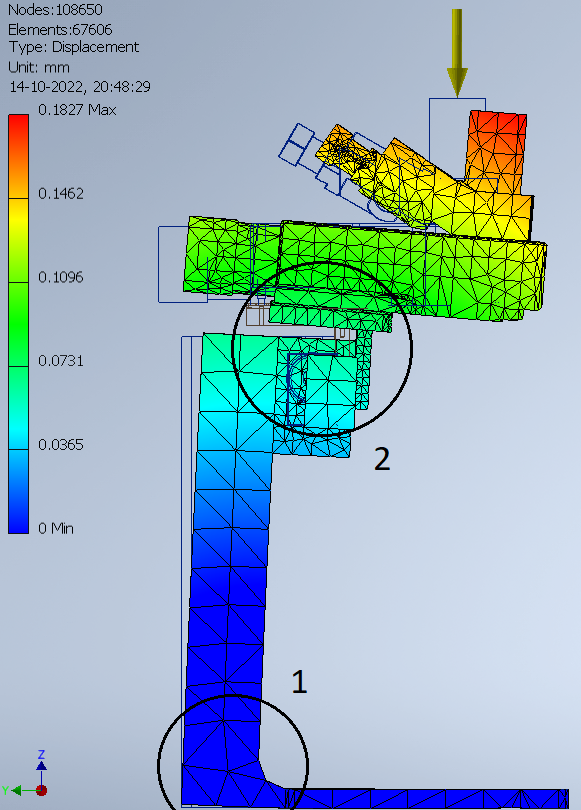
\includegraphics[width=0.8\textwidth]{img/rigidity_simulation/study_4.png}
    \caption{100 N pressing force on a static point on the microscope. To reduce displacement a $30\mathrm{mm}$ fillet was added between the base-plate and stand \textbf{(1)}. To reduce cantilever effects a custom $90^\circ$ angle bracket \textbf{(2)} was created to position the microscope head above the stand. By using the adaptions the the maximum displacement is reduced to $183\mathrm{\mu m}$. By R. Stoelwinder }
    \label{fig:disp_study4}
  \end{minipage}
  \hfill
  \begin{minipage}[b]{0.45\textwidth}
    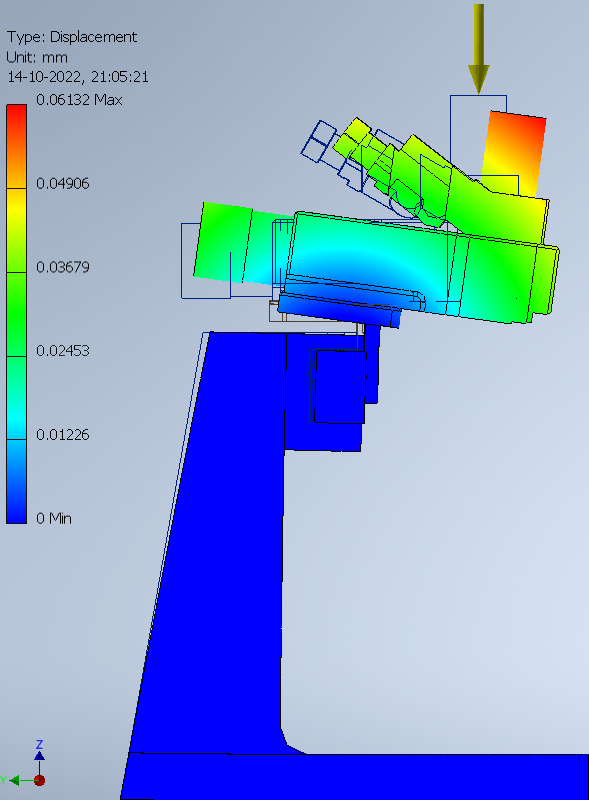
\includegraphics[width=0.8\textwidth]{img/rigidity_simulation/study_7.png}
    \caption{100N pressing force on a static point on the microscope head. To reduce the the maximum displacement the thickness of the base-plate is increased from $20\mathrm{mm}$ to $50\mathrm{mm}$ and the stand shape changed to a solid trapezium geometry, reducing the maximum displacement to $50\mathrm{\mu m}$. By R. Stoelwinder}
    \label{fig:disp_study7}
  \end{minipage}
\end{figure}

The first iteration of the microscope stand, visible in figure \ref{fig:disp_study4} is based on the Olympus SZ-STL microscope stand \todo{referentie naar onderdeel toevoegen} in example configuration 1 \todo{referentie invoegen}. \todo{Mention the used material so the properties are tracable}
To reduce the cantilever effect of the microscope head on the stand the choice was made to use a $90^\circ$ bracket to position the microscope head on top of the stand instead of in frond of it like the default Olympus configuration \todo{referentie naar config 1 invoegen}. 
A fillet was also added to the connection between the base and the vertical bar to improve the rigidity of the connection.\\

After the additions in figure \ref{fig:disp_study4} it can be seen that the weakest point in the stand is now the vertical extrusion part of the stand that holds the microscope. 
To improve the rigidity of the stand the trapezium shape was chosen for it's rigid geometry.
From the simulation in figure \ref{fig:disp_study4} it is known that the connection between the base and the stand is a possible weak point. 
To prevent the connection between the base and the stand from becoming a weak point again after adding the fillet we have chosen to also thicken the base.
In combination with using a solid aluminum profile instead of the $1 \mathrm{cm}$ extrusion profile the deflection under load was reduced further but still there are clear weak points that can be resolved as can be seen in figure \ref{fig:disp_study7}.\\


\begin{figure}[H]
  \centering
  \begin{minipage}[b]{0.45\textwidth}
    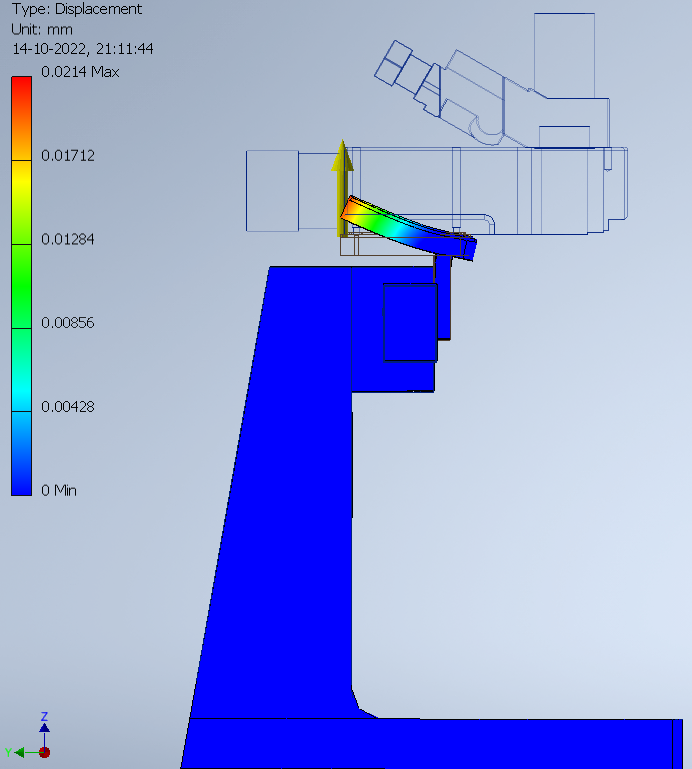
\includegraphics[width=\textwidth]{img/rigidity_simulation/study_8.png}
    \caption{100N pulling force on a static point on the microscope bracket. When comparing to figure \ref{fig:disp_study7} it can be seen that the bracket is indeed the weak point of the stand causing a $21\mathrm{\mu m}$ displacement. By R. Stoelwinder}
    \label{fig:disp_study8}
  \end{minipage}
  \hfill
  \begin{minipage}[b]{0.45\textwidth}
    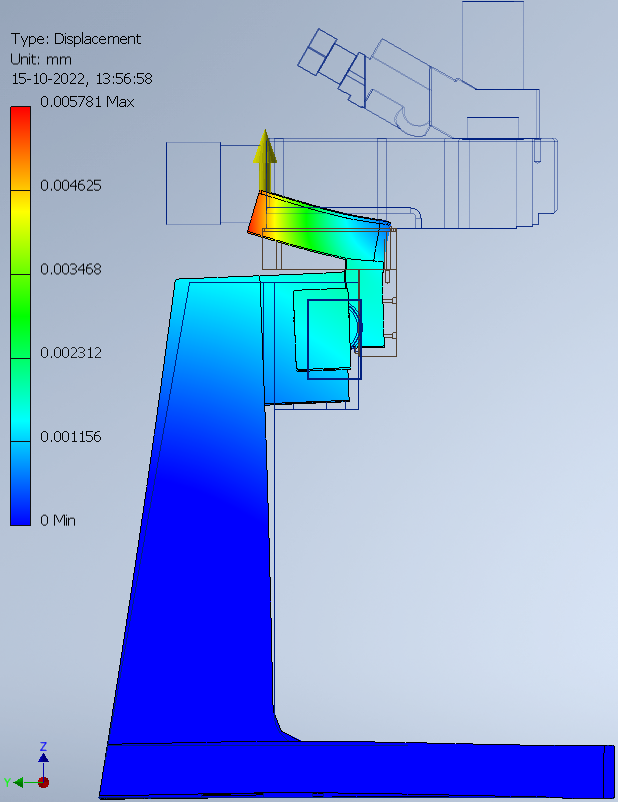
\includegraphics[width=1\textwidth]{img/rigidity_simulation/study_10.png}
    \caption{100 N pulling force on a static point on the corner-plate. To reduce the maximum displacement the thickness of the corner plate is increased from  $20\mathrm{mm}$ to $40\mathrm{mm}$, reducing the maximum displacement to $6\mathrm{\mu m}$. By R. Stoelwinder }
    \label{fig:disp_study10}
  \end{minipage}
\end{figure}

As seen in figure \ref{fig:disp_study7} the new weak point has become the bracket that was added in figure \ref{fig:disp_study4}.
To remove the influence of the microscope head on the bending of the bracket a new simulation was made of the model in figure \ref{fig:disp_study7} without the microscope head has been made (see figure \ref{fig:disp_study8})
The simulation in figure \ref{fig:disp_study8} clearly shows that the bracket is indeed the new weak point of the stand. 
By increasing the thickness of the bracket and fabricating the bracket out of a solid block the deflection was reduced further.
The final reached deflection of $6\mathrm{\mu m}$ is sufficient for the further development of the instrument as the simulations are made using a force of $100\mathrm{N} = 10.2 \mathrm{kg}$ which is a significantly higher force than can be expected from an amplitude driven vibration so the deflection will not be reached in practice.\\

The final design for the microscope stand can be seen in figure \ref{fig:trap_stand}, the schematic can be found in appendix \ref{doc:tech_base} and \ref{doc:tech_trap_mount}.\\

\begin{figure}[htp]
  \centering
  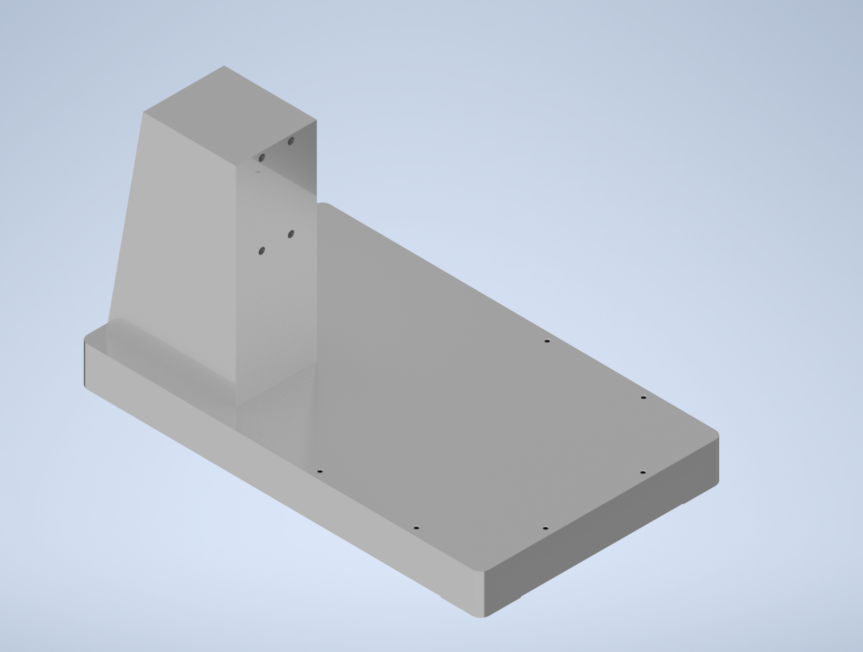
\includegraphics[width=0.5\textwidth]{img/stand_design/microscope_stand.png}
  \caption{The final design of the microscope stand. By R. Stoelwinder}
  \label{fig:trap_stand}
\end{figure}

\clearpage
\subsection{Mask design}
the mask consists of two major parts: the mask holder which holds the stamping polymer and the stages which are used to align the flake on the mask with the target flake.
The design of the mask holder is fairly straight forward, the mask should be as rigid as possible while minimizing the cantilevers in the design.
To make the stack of stages used to manipulate the mask more stable a custom bracket was fabricated to position the mask near the center of the stage stack.
For the final design and assembly of the mask holder see appendix \ref{doc:summary_assembly}\\

\subsection{Sample holder design}
The main task of the sample holder, as the name implies, is to hold the sample in position. 
The sample holder is also used to change the temperature of the sample.
Like the rest of the instrument, it is important to make the sample holder as rigid as possible to ensure that the vibrations of the mask, camera and sample remain in phase.\\

Over the duration of this project, the first prototype of the sample holder was fabricated and plans were made for the follow-up design. 
Both versions of the sample holder consist of three parts: The sample bed (see figure \ref{fig:prototype_sample_holder}), insulation layer and the spacer bus (see appendix \ref{doc:tech_stages}).\\

\subsubsection{Sample bed}

\begin{figure}[H]
  \centering
  \begin{minipage}[b]{0.45\textwidth}
    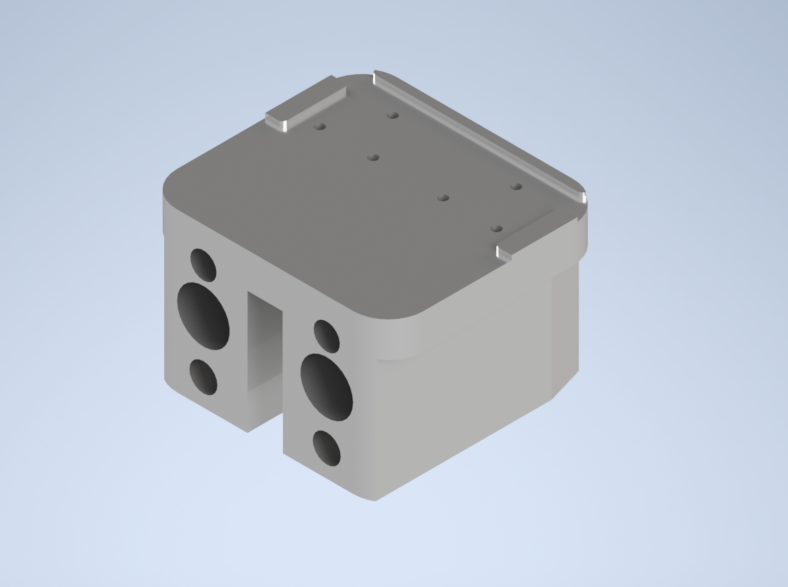
\includegraphics[width=1.17\textwidth]{img/sample_holder_and_mask/prototype_sample_block.png}
    \caption{Autodesk Inventor render of the prototype sample holder prototype. Design by R. Stoelwinder \& B. Klein Ikkink}
    \label{fig:prototype_sample_holder}
  \end{minipage}
  \hfill
  \begin{minipage}[b]{0.45\textwidth}
    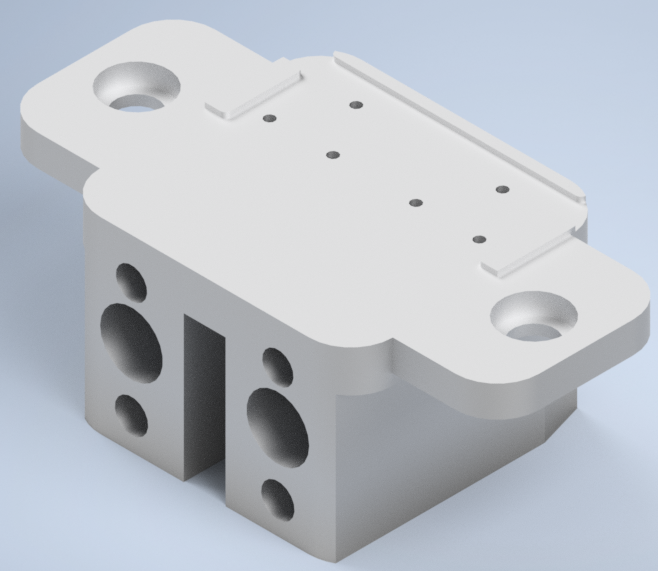
\includegraphics[width=1\textwidth]{img/sample_holder_and_mask/sample_holder_render_bas.png}
    \caption{Autodesk Inventor render of the next version sample holder. Design by R. Stoelwinder \& B. Klein Ikkink}
    \label{fig:next_sample_holder}
  \end{minipage}
\end{figure}

The sample bed contains the necessary components to bring the sample to the desired temperature between $0$ and $200^\circ$C a heating coil and TEC element are used. 
The bed is heated using the heating coil and cooled bys using the TEC element to transfer heat from the sample bed to the spacer bus (for component id's see appendix \ref{ap:used_components}).
Due to the temperature difference between the sample bed and spacer cylinder after cooling an isolation layer is needed to prevent the heat from flowing back into the sample bed.
For this purpose an PEEK isolation layer is used as PEEK has the needed thermal insulating properties and can be machined relatively easy \cite{lingPolyetherEtherKetone2020}.\\

During the testing of the prototype some problems came to light, mainly the rigidity of the connection between the spacer bus and the sample bed and the long term characteristics of the used thermal compound.
As seen in figure \ref{fig:prototype_sample_holder} the sample bed is only attached to the isolation layer by press fit, this is sufficient for testing purposes but not for usage by the end-user.
Due to the method of attachment in combination with the used thermal compound it is also not possible to reliably level the sample bed.
A consequence this can be that the instrument behaves differently than the end-user expects, for example, when rotating the sample the sample will get out of focus.
Due to degradation of the thermal compound the heat transfer characteristics of the used TEC element can also degrade due to lesser contact with the sample bed, this will influence the behavoir of the used PID controller.\\

A significant part of the leveling issue can be resolved to press the sample bed onto the isolator with more force.
To address the leveling issue the design showed in figure \ref{fig:next_sample_holder} was created, which features two new mounts that can be used as screw holders for PEEK clamping screws.
While this design shows improvement the mass should still be reduced as much as possible to minimize the heat capacity in the sample bed (see equation \ref{eq:heat_energy_in_cilinder}).
This can be done by reducing the amount of mounting points on the sample bed, the vacuum tube mounts can be reduced to one (instead of one for each sample position), the same applies for the heating coil.
These adaptions will reduce the mounting points from six to three (thermocouple, PT100, vacuum tube) while also making it possible to make the sample bed smaller.

For the thermal compound it is recommend to look for a compound that does not degrade over time, for example liquid metal thermal compound, this is easier said than done as most generic liquid metal compounds contain Gallium, which reacts with the used aluminum for fabricating the sample bed.\\

Due to time constraints is was not possible to fabricate the next iteration of the sample holder and all tests were performed on the prototype sample holder.\\


\subsubsection{Spacer bus}

To be able to meet the criteria set in \ref{ch:criteria} the sample bed has to be able to cool down to $20^\circ$C, this means that the heat energy from the sample bed has to be transported to the cylinder and dissipated.

\todo{Isert a paragraph about the used PID settings for testing}


\begin{equation}
  Q(x,t) = CmT(x, t) \rightarrow T(x,t) = \frac{Q(x, t)}{Cm}
  \label{eq:heat_energy_in_cilinder}
\end{equation}

\begin{equation}
  \frac{\mathrm{d}Q}{\mathrm{d}t} = -KA\frac{\delta T(x, t)}{\delta {x}}
  \label{eq:fourrier_law}
\end{equation}

\begin{equation}
  \frac{\delta{T(x,t)}}{\delta t} = -\frac{K}{C\rho}\frac{\delta^{2} T(x, t)}{\delta x^2}
  \label{eq:heat_equation}
\end{equation}

A model of the heat distribution in the spacer bus can be made by combining equation \ref{eq:heat_energy_in_cilinder} with equation \ref{eq:fourrier_law} known as Fourier's Law, resulting in equation \ref{eq:heat_equation}, also known as the heat equation 
The code used to generate the model can be found in appendix \ref{ap:cylinder_mode}

\begin{figure}[H]
  \centering
  \begin{minipage}[b]{0.45\textwidth}
    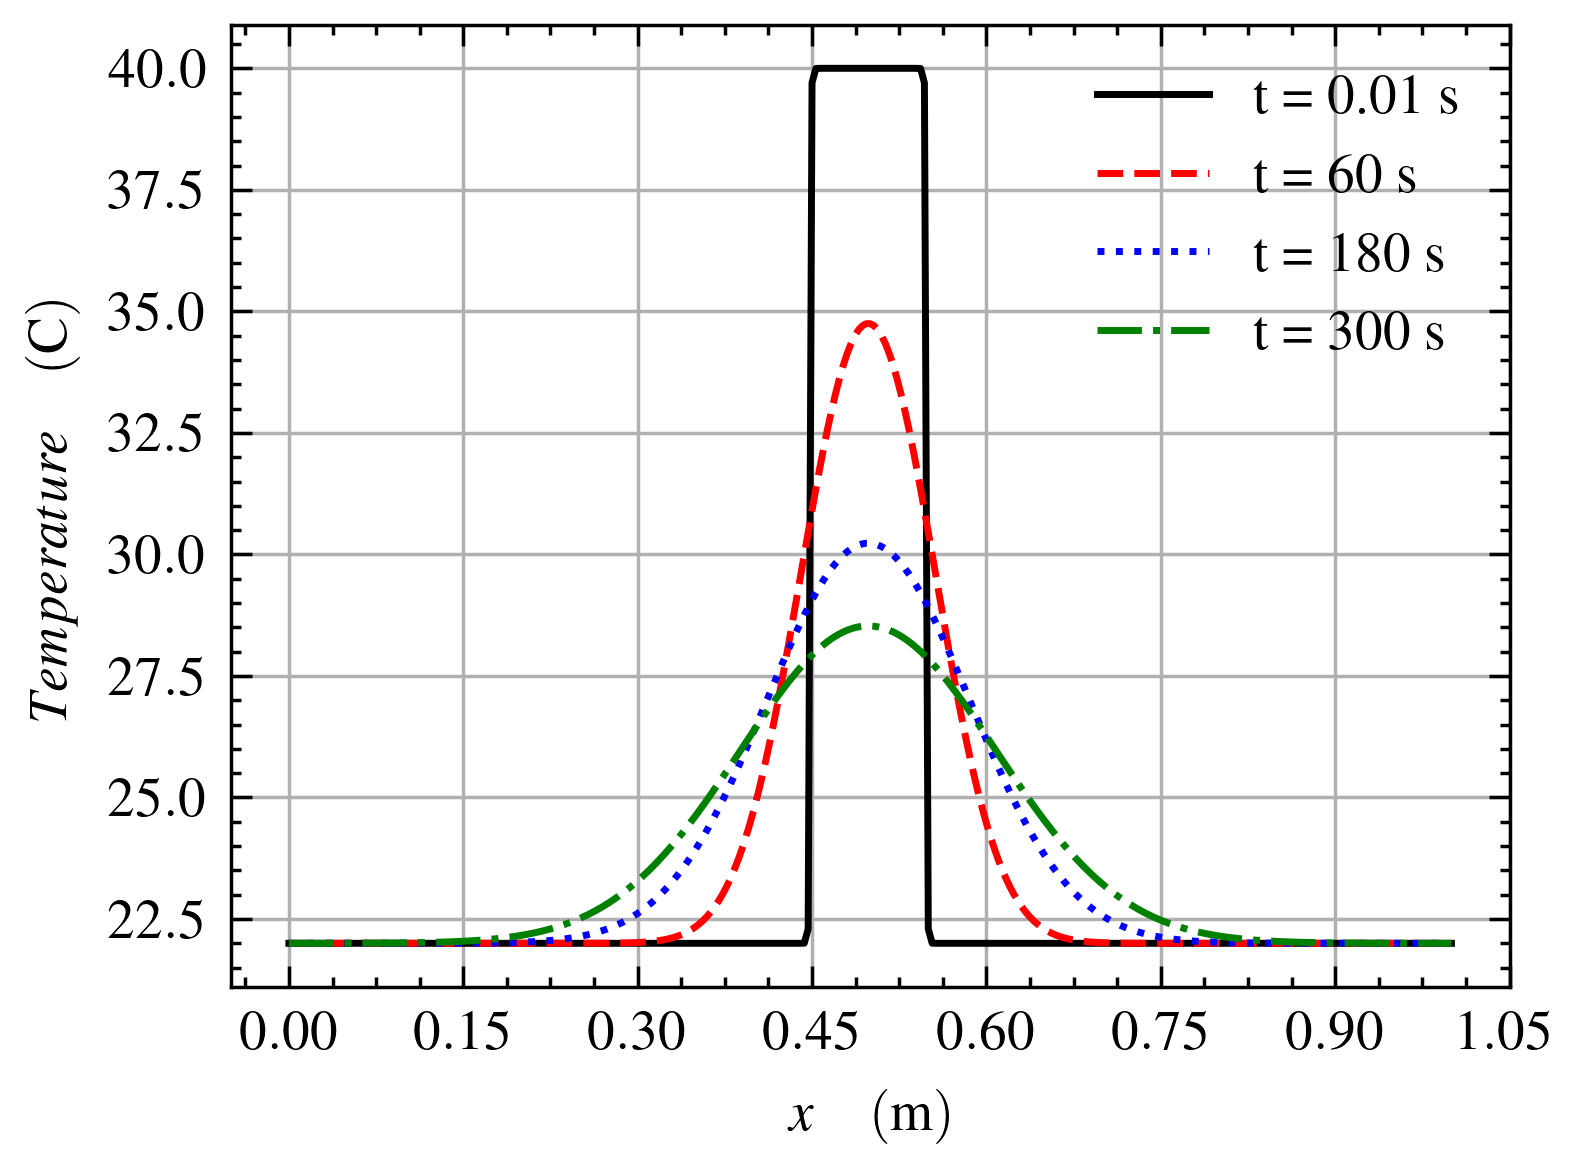
\includegraphics[width=\textwidth]{img/sample_holder_and_mask/solid_cylinder_model.png}
    \caption{A model approximating the heat distribution in the spacer bus after dissipating heat to the surrounding air, assuming the heat transfer does not introduce significant convection in the air according to equation \ref{eq:heat_equation}. $T_{0N} = 23^\circ$C, $T_{0al} = 60^\circ$C.}
    \label{fig:solid_cilinder model}
  \end{minipage}
  \hfill
  \begin{minipage}[b]{0.45\textwidth}
    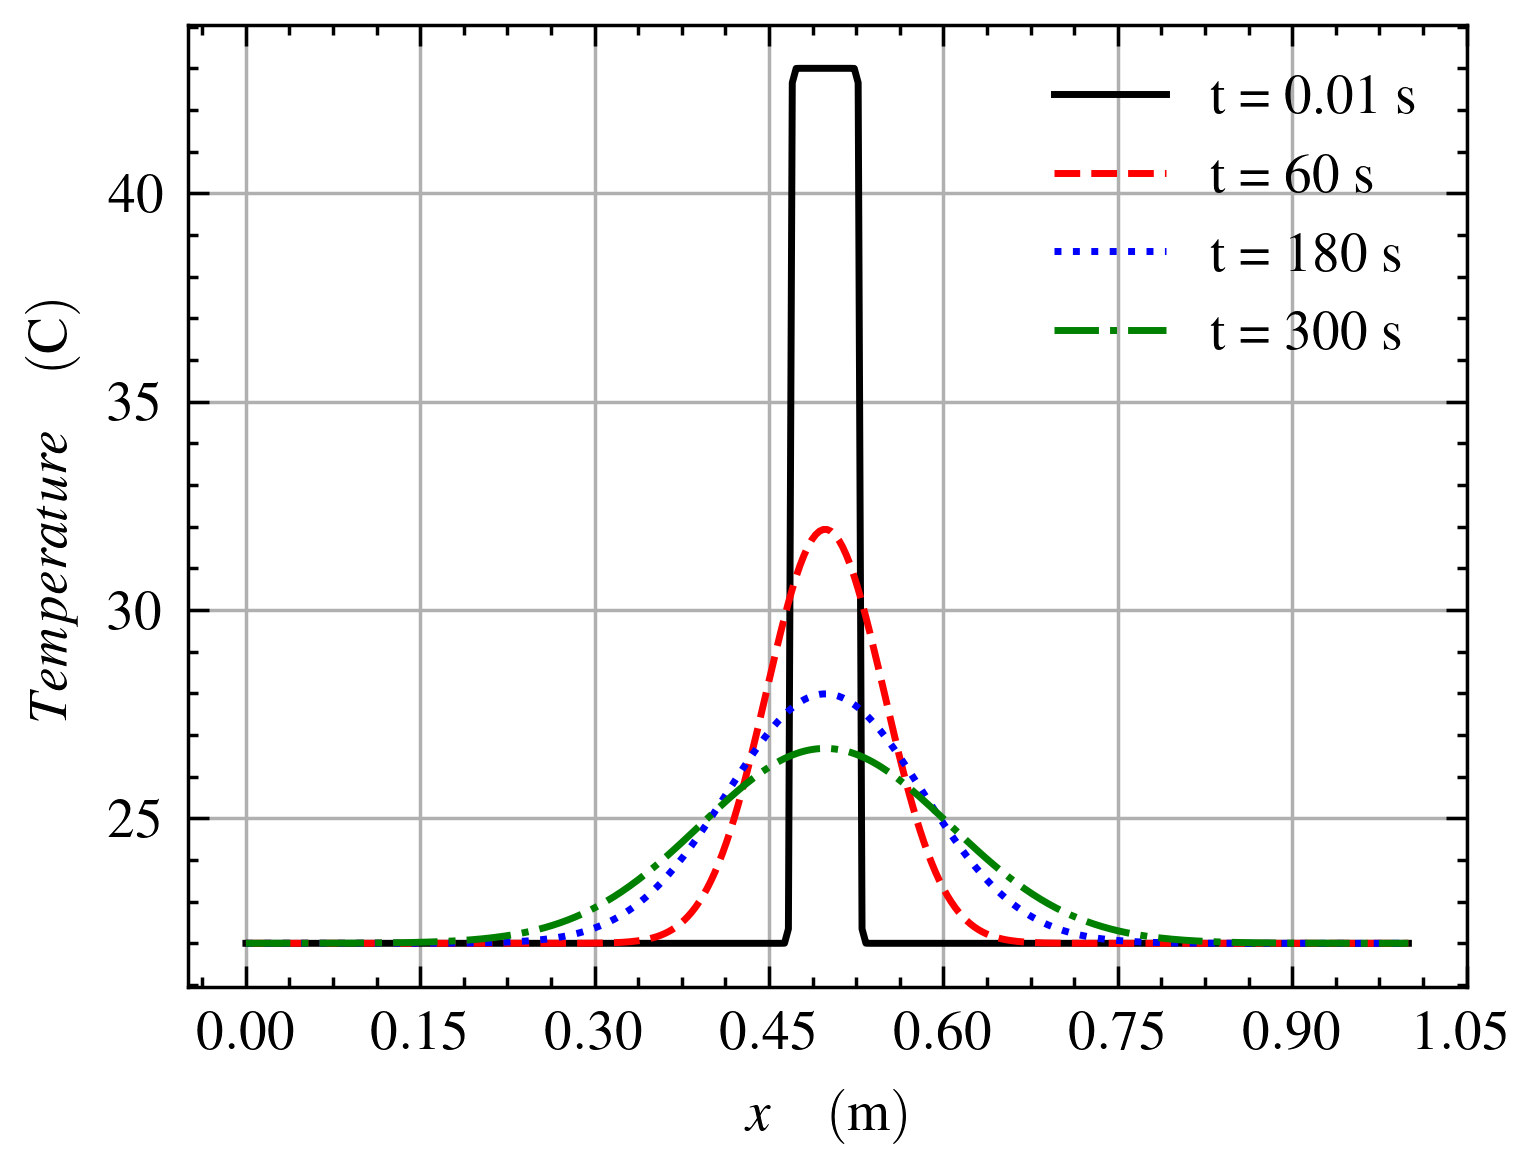
\includegraphics[width=1\textwidth]{img/sample_holder_and_mask/reduced_cylinder_model.png}
    \caption{A model approximating the heat distribution in the spacer bus with reduced mass after dissipating heat to the surrounding air, assuming the heat transfer does not introduce significant convection in the air according to equation \ref{eq:heat_equation}. $T_{0N} = 23^\circ$C, $T_{0al} = 40^\circ$C, due to the capacity of the used TEC element the max $\Delta T$ between the cylinder and sample bed that can be reached is $\pm 40^\circ$C so the maximum temperature the cylinder can reach while keeping the performance of the instrument is $40^\circ$C \ref{eq:heat_energy_in_cilinder}.}
  \end{minipage}
\end{figure}


\todo{keuze voor peek en mica onderbouwen}
\todo{CAD schema van de sample holder invoegen}
% Insert the temperature graph and the cad schematic of the sample holder
\begin{figure}[H]
  \centering
  \begin{minipage}[b]{0.45\textwidth}
    %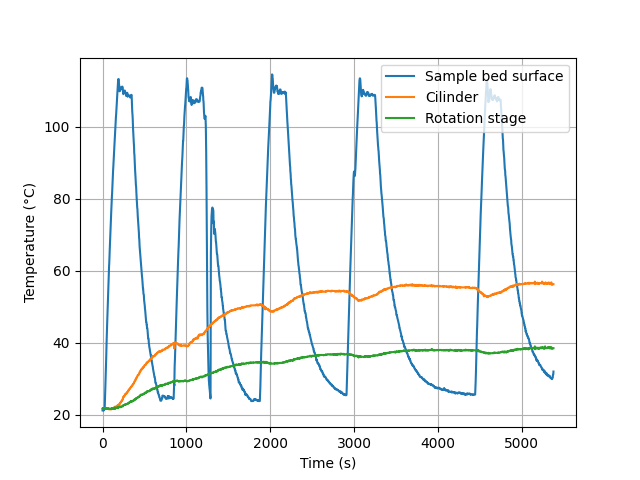
\includegraphics[width=\textwidth]{img/sample_holder_and_mask/temp_cycling.png}
    \caption{Temperature graph of the sample holder when simulating workload by heating to 110 degrees and cooling down to ambient temperature ($25^\circ$) while waiting for 120 seconds when the level is reached.}
    \label{fig:temperature_graph}
  \end{minipage}
  \hfill
  \begin{minipage}[b]{0.45\textwidth}
    %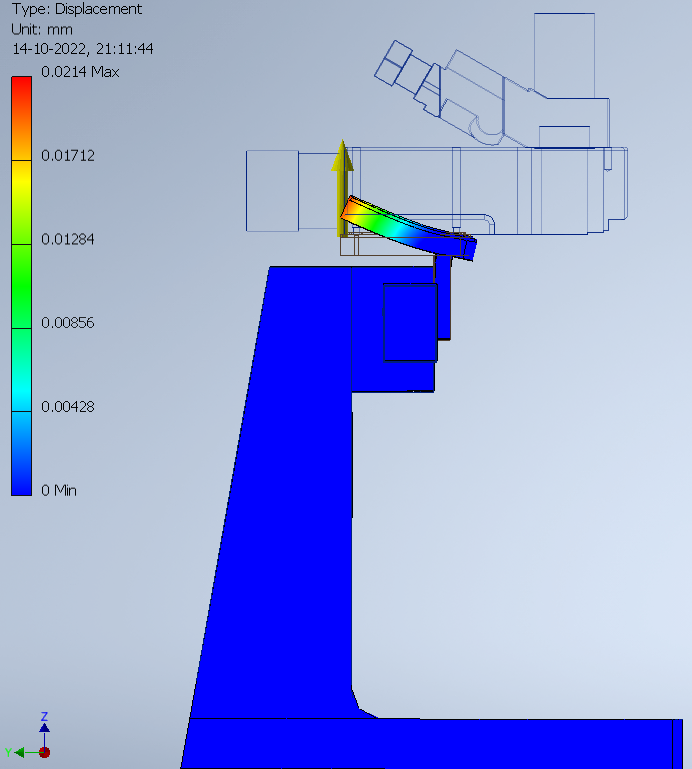
\includegraphics[width=1\textwidth]{img/rigidity_simulation/study_8.png}
    \caption{CAD schematic of the sample holder. By R. Stoelwinder. The sample holder prototype consists of 4 major parts. 1. The sample bed, which contains a heating coil, TEC element, thermocouple and PT100 sensor. 2. The sample isolation layer. This is a shroud fabricated out of PEEK}
    \label{fig:CAD_sample_holder}
  \end{minipage}
\end{figure}

\subsection{Stage automation}

\subsubsection{Mask stages}

\todo{CAD schema van de mask holder invoegen}
\begin{figure}[H]
  \centering
  \begin{minipage}[b]{0.45\textwidth}
    %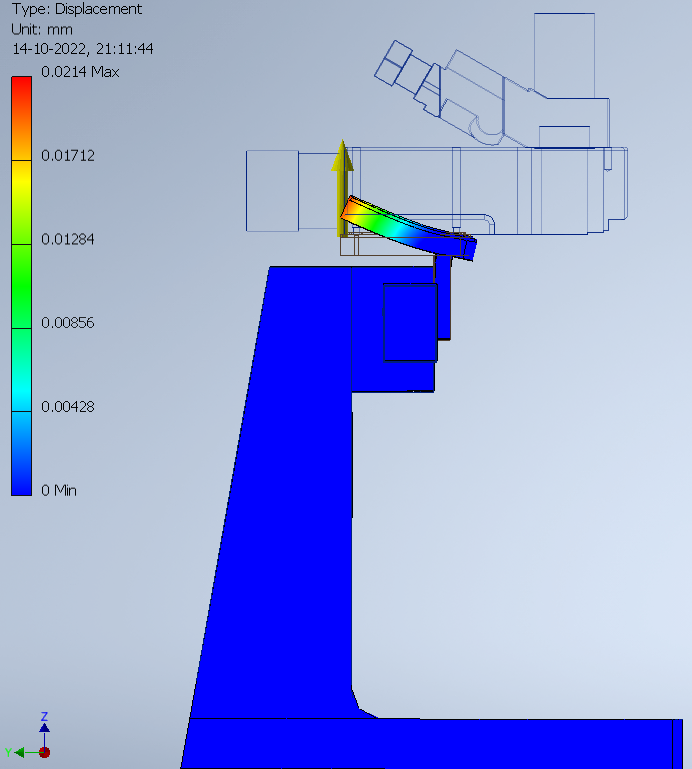
\includegraphics[width=\textwidth]{img/rigidity_simulation/study_8.png}
  \end{minipage}
  \hfill
  \begin{minipage}[b]{0.45\textwidth}
    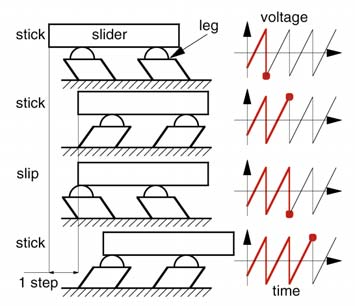
\includegraphics[width=1\textwidth]{img/sample_holder_and_mask/Stick-slip-piezo-actuator-operation-principle.png}
    \caption{Operating principle of a slip-stick actuator mechanism 
    \cite{mazerollePositioningHandlingMeasuring2003}}
    \label{fig:slip_stick_principle}
  \end{minipage}
\end{figure}

\subsubsection{Sample stages}

\subsubsection{Course stages}
\todo{CAD van bracket invoegen}

for this project the base xy stage (\todo{ref naar optosigma stage invoegen}) has to be automated, this will developed in house in collaboration with LU FMD and ELD. 

The stages were automated using NEMA17 stepper motors \todo{citation invoegen}, and optical end-stops.
The stepper motors and end-stops are controlled by the controller developed by ELD.
The contents and used techniques in the control box are out of the scope for this report.

The first prototype bracket makes it possible to test the complete system and work out implementation bugs. 
It is recommended to create further iterations of the bracket as the current version can flex $\pm 3mm$ and this has a detrimental effect on the rigidity of the base xy stage, this because the stages are held in place by the stepper motor. 
Furthermore it is also recommended to replace the ball bearings in the spindles as these were damaged during fabrication and the spindle is now only held in place by the stepper motor

\subsection{Stage calibration}
Due to the mechanisms used in some of the actuators it is not possible to calibrate all the staged,
nor is this needed for the application. 
The stages that cannot be calibrated are the x, y, and z axis of the mask due to the used slip-stick mechanism (see figure \ref{fig:slip_stick_principle}). 

The slip stick mechanism makes it possible to use Piezo actuators with high resolution for an unbound range.
The drawback is that due to the slip stick mechanism (friction based) the actuator has a position uncertainty of \todo{positie uncertainty invoegen} and a step uncertainty of \todo{step variatie invoegen}.

\subsection{Software}
Because one of the main criteria of the project is flexibility and modularity this has to be taken in consideration from the beginning. 
This means the project needs to be created in a structured and standardized way using design patterns and a modular architecture.

\subsubsection{Architecture}
As a main architecture a web application inspired framework is used. 
This means that the system consist of three major components: Frontend, Middleware and backend. 
Using standard design patterns makes getting to know the code and editing it less cumbersome and error prone for future developers.
An overview of the system flow can be seen in figure \ref{fig:software_architecture}

\todo{laatste pijlen in de correcte richting zetten}
\begin{figure}[htp]
  \centering
  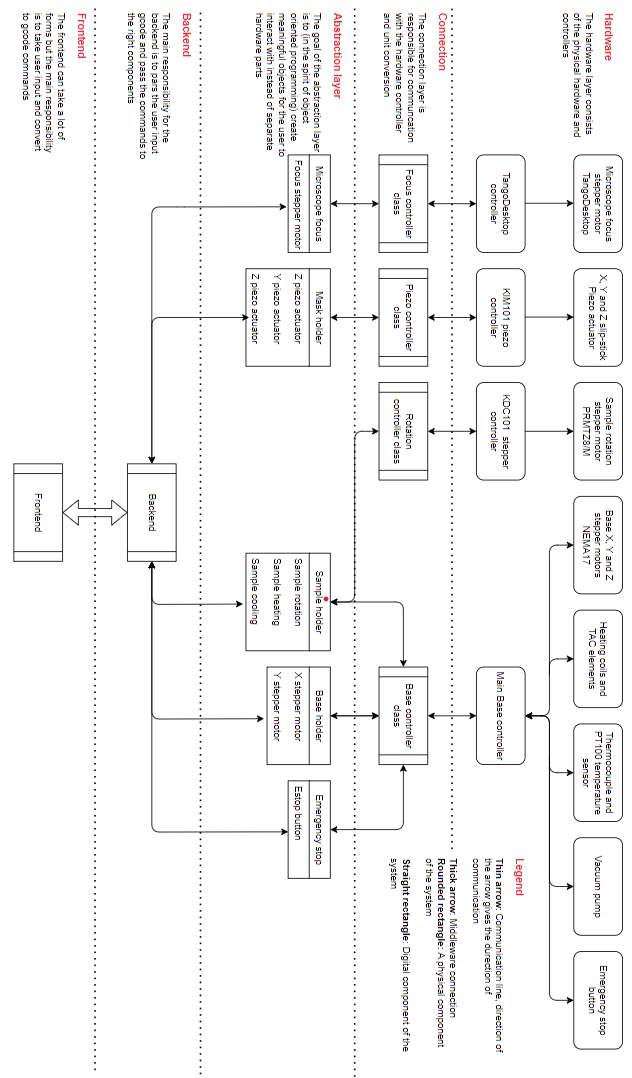
\includegraphics[width=0.8\textwidth]{img/design_cycle/code_flow.png}
  \caption{Software flow of the project.}
  \label{fig:software_architecture}
\end{figure}

\subsubsection{Frontend}
The frontend is the part of the system that is visible to the user.
This part of the system is responsible for the user interface and the communication with the middleware.
The system has two pre made interface options: GUI and TUI.
For operators of the system it is recommended to use the GUI as no knowledge of the command set is needed and safety features like thermal-runaway and forbidden areas are enabled.
For developers it is recommended to use the TUI as it is more flexible and allows for more control over the system.

The GUI is created using QT6 with Pyside6 bindings \todo{citation invoegen} to ensure interoperability between different operating systems and detailed documentation for future developers.

The TUI consists of a simple loop that pushes the Gcode commands to the backend and uses a thread to monitor the backend response.

\subsubsection{Middleware}
The middleware is a method that can be used to communicate between the frond and backend. 
The middleware base class contains all the base methods needed for the system to work with a middleware method.
The system contains two default middleware methods: The processing pipe, which is used for when the backend runs on the same computer as the frontend but on a separate core (it is strongly discouraged to run the backend on the same core as the frontend as this makes the backend behavior depend on core workload.) 
The second method is the serial method and is based on the PySerial library \todo{citation invoegen} and is used when the backend runs a different computer than the frontend.
The serial middleware method can be easily adapted to work with wireless serial communication but this is discouraged as this method is more prone to errors.

\subsubsection{Backend}
The backend is the part of the system that is responsible for the communication with the hardware and the middleware and managed the object the user can interact with (sample holder, mask holder, etc.)
The backend accepts all classes that inherit from their respective base class and abide the programming guidelines \todo{referentie naar docs toevoegen}

Due to time constraints it was not possible to develop the backend to run on unix based systems

\todo{Add a snippet of the important functions (excecution loop and command loop)}

\todo{stukje over FTDI issue tovoegen}
\todo{stukje over voordeel van runnen op IO controller toevoegen}

\subsubsection{Forbidden areas}
To prevent the system from damaging itself or the sample it is important to prevent the system from moving to certain areas in certain states.

Phase space variables (system attributes):
\begin{itemize}
    \item Position of all the axis*
    \item Velocity of all the axis
    \item Acceleration of all the axis
    \item Sample temperature
    \item Sample heating and cooling ramp
\end{itemize}

This means the phase space will consist of 21 dimensions, where each dimension represents the current value of a system attribute.

First the phase space is bordered off by the hardware limitations like maximum velocity, minimal reproducible step size, range, etc.
Further forbidden areas are studied using a fractional factorial design to determine the most important variables that influence the system.

The forbidden areas will be determined using a fractional factorial design with the following parameters

(see excel file)




\clearpage
\section{Conclusion}

\section{Discussion}


\newpage
\begin{multicols*}
{2}[\printbibheading]
    \AtNextBibliography{\footnotesize}
    \printbibliography[heading = none]
    \addcontentsline{toc}{section}{Bibliography}
\end{multicols*}

\clearpage
\appendix

\section{Hardware functional decompositions}
\label{ap:hardware_functional_decomposition}
\begin{figure}[htp]
  \centering
  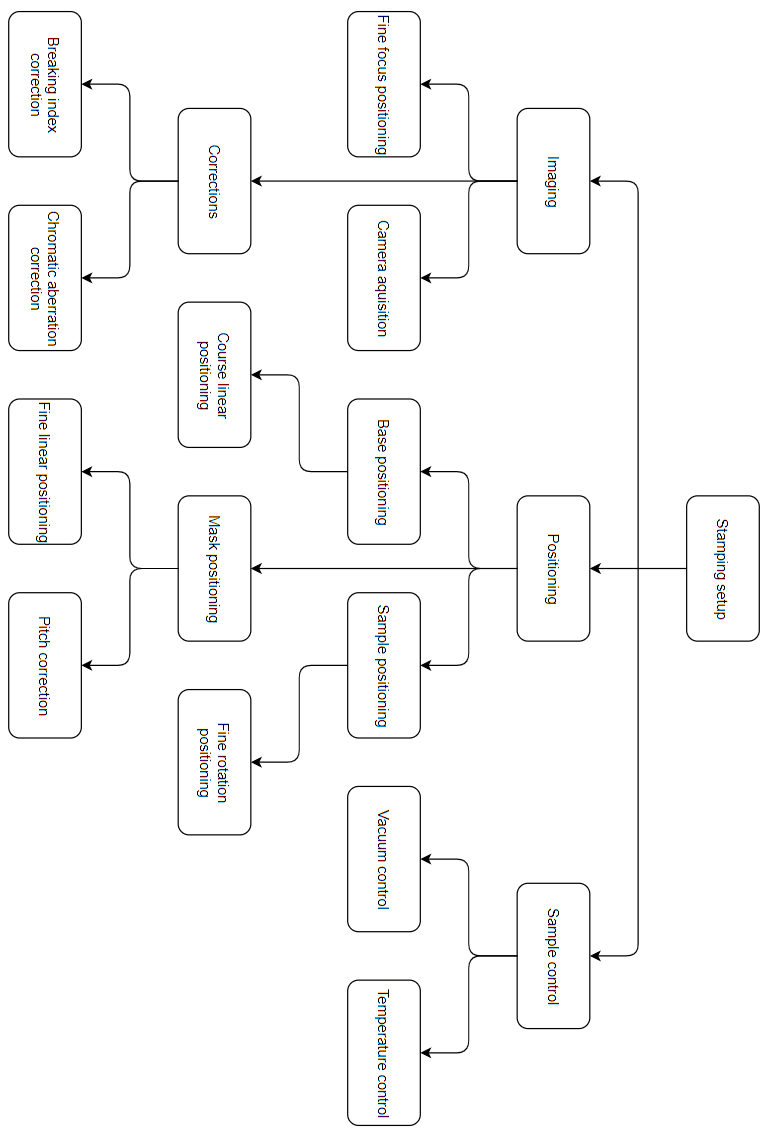
\includegraphics[width=0.7\textwidth]{img/design_cycle/functional_decomposition_hardware.png}
  \caption{Functional decomposition of the hardware for the project.}
  \label{fig:functional_decomposition_hardware}
\end{figure}

\clearpage
\section{Software functional decomposition}
\label{ap:software_functional_decomposition}
\begin{figure}[htp]
  \centering
  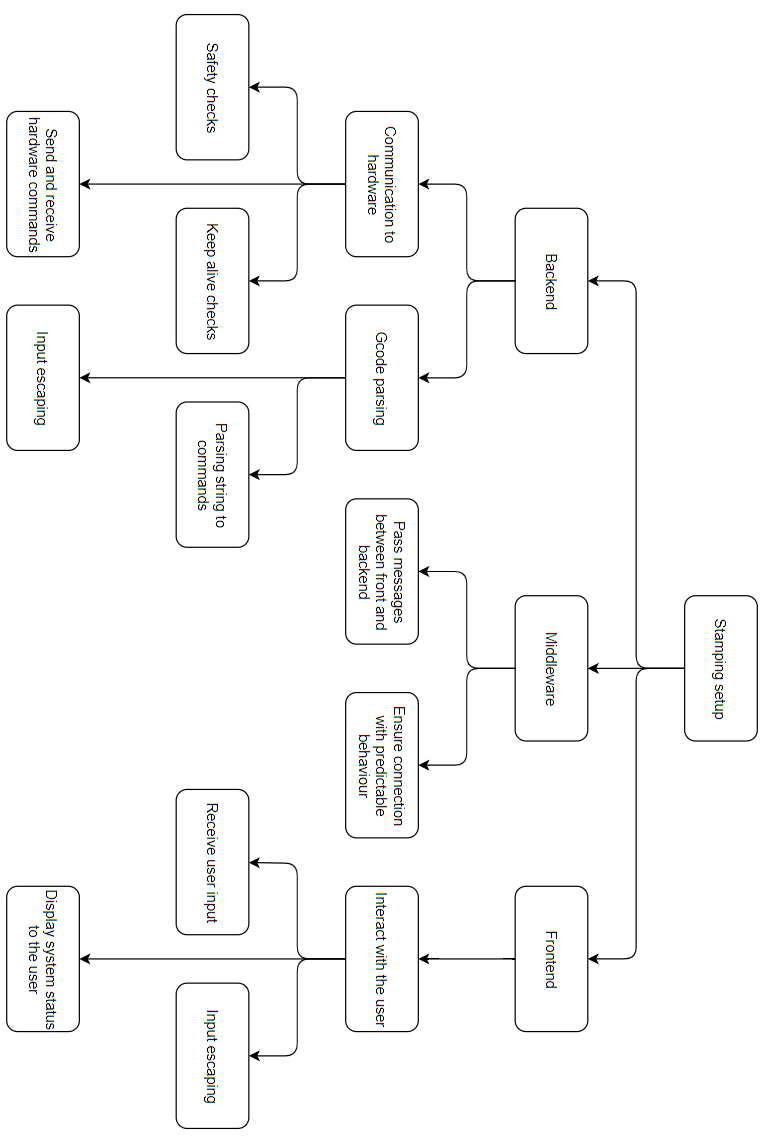
\includegraphics[width=0.7\textwidth]{img/design_cycle/functional_decomposition_software.png}
  \caption{Functional decomposition of the software for the project.}
  \label{fig:functional_decomposition_software}
\end{figure}

\clearpage
\section{Used components}
\label{ap:used_components}
For this project the following commercial products were used.
\begin{itemize}[noitemsep]
  \item Microscope:
  \begin{itemize}[noitemsep]
    \item Manual Illuminator: BX3M-RLA-S
    \item LED light source: BX3M-LEDR 
    \item LED power supply:  BX3M-PSLED
    \item Camera: DP23-CU
    \item Illuminator holder: BXFM-ILHSPU
    \item Widefield trinocular tube: U-TR30-2
    \item Manual nosepiece: U-D6BDRE
  \end{itemize}
  \item Stages:
  \begin{itemize}[noitemsep]
    \item Thorlabs MT1/M  \cite{ThorlabsMT11}
    \item Thorlabs MT402/M \cite{ThorlabsMT402RightAngle}
    \item Thorlabs XRNG1/M \cite{ThorlabsXRNG1QuickConnect}
    \item Thorlabs XRNR1/M \cite{ThorlabsXRNR1O56}
    \item Thorlabs XRN-B1/M \cite{ThorlabsXRNB1Base}
    \item OptoSigma TSM-3003
    \item OptoSigma TAMC-30302
  \end{itemize}
  \item Actuators:
  \begin{itemize}[noitemsep]
    \item Thorlabs PIA13
    \item Thorlabs PRMTZ8/M
    \item \todo{Focus motor invoegen}
  \end{itemize}
  \item Controllers:
  \begin{itemize}[noitemsep]
    \item Thorlabs KIM101 piezocontroller
    \item Thorlabs KDC101 stepper motor controller
    \item TangoDesktop 1 axis stepper motor controller
  \end{itemize}
\end{itemize}

\clearpage
\section{Vibration measurement in VDWSF Lab}
\label{ap:vibrational_measurement}

\begin{figure}[htp]
  \centering
  \begin{minipage}[b]{1\textwidth}
    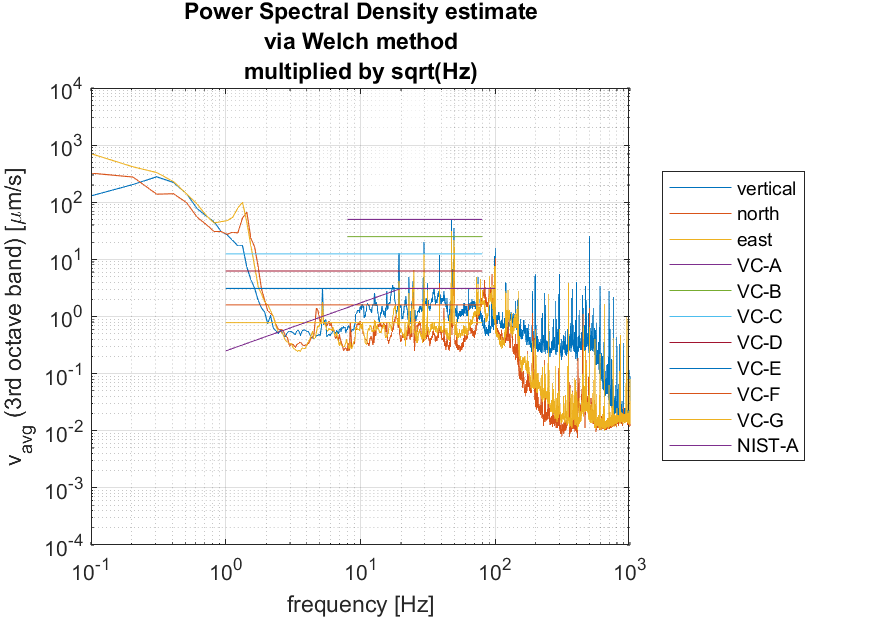
\includegraphics[width=\textwidth]{img/resonance/geophone_measurement_position_1.png}
    \caption{Measured vibration data in the Van der Waals Stacking Facility laboratory on the position of the stacking instrumentation. By J. Scheffer}
    \label{ap:GEOPhone_measurement}
  \end{minipage}
\end{figure}


\clearpage
\section{Cylinder temperature distribution model}
\label{ap:cylinder_mode}
\lstinputlisting[language=Python]{code/cylinder/model.py}

\clearpage
\section{Complete setup schematics}

This section contains the technical information on the fabricated components of the setup.
All components are made of Al6061 if not mentioned otherwise.
All designs were created in collaboration with R. Stoelwinder from LU FMD

\label{ap:complete_schematics}
\begin{figure}[tp]
  \centering
  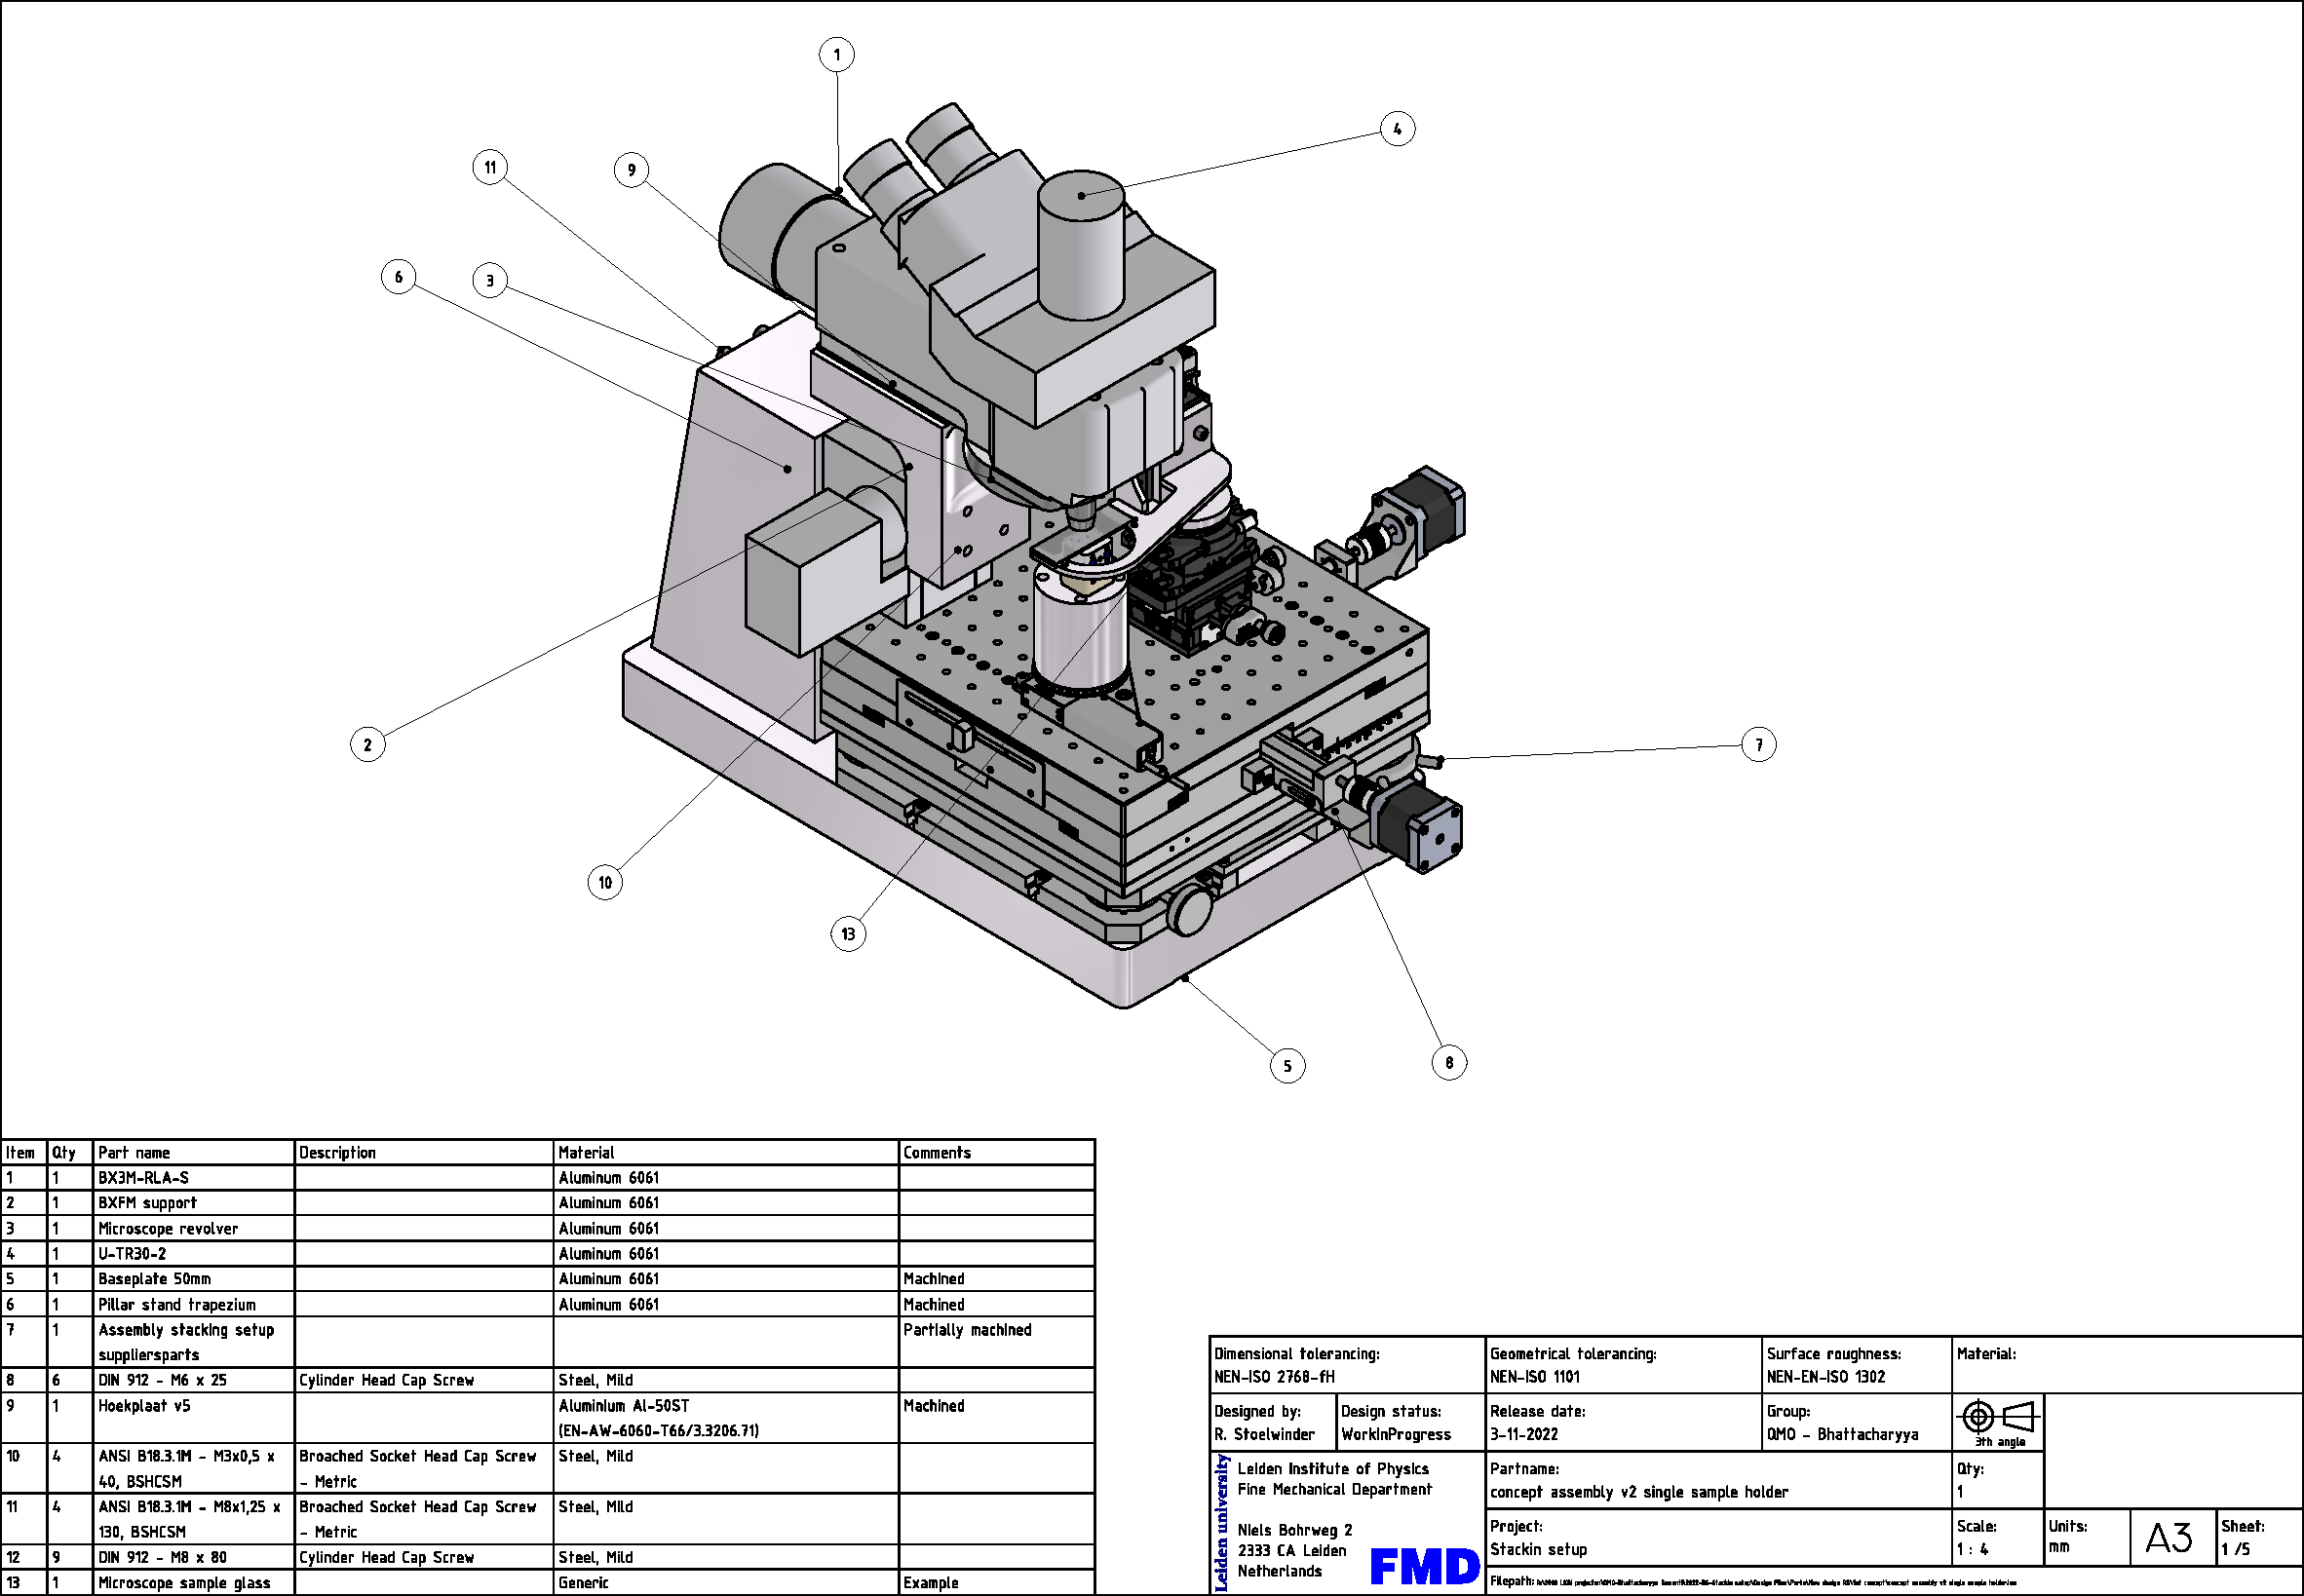
\includegraphics[angle=90,origin=c,width=\textwidth]{img/cad/pag1}
  \caption{Technical drawing of instrument design. By R. Stoelwinder}
  \label{doc:summary_assembly}
\end{figure}

\clearpage
\begin{figure}[htp] 
  \centering
  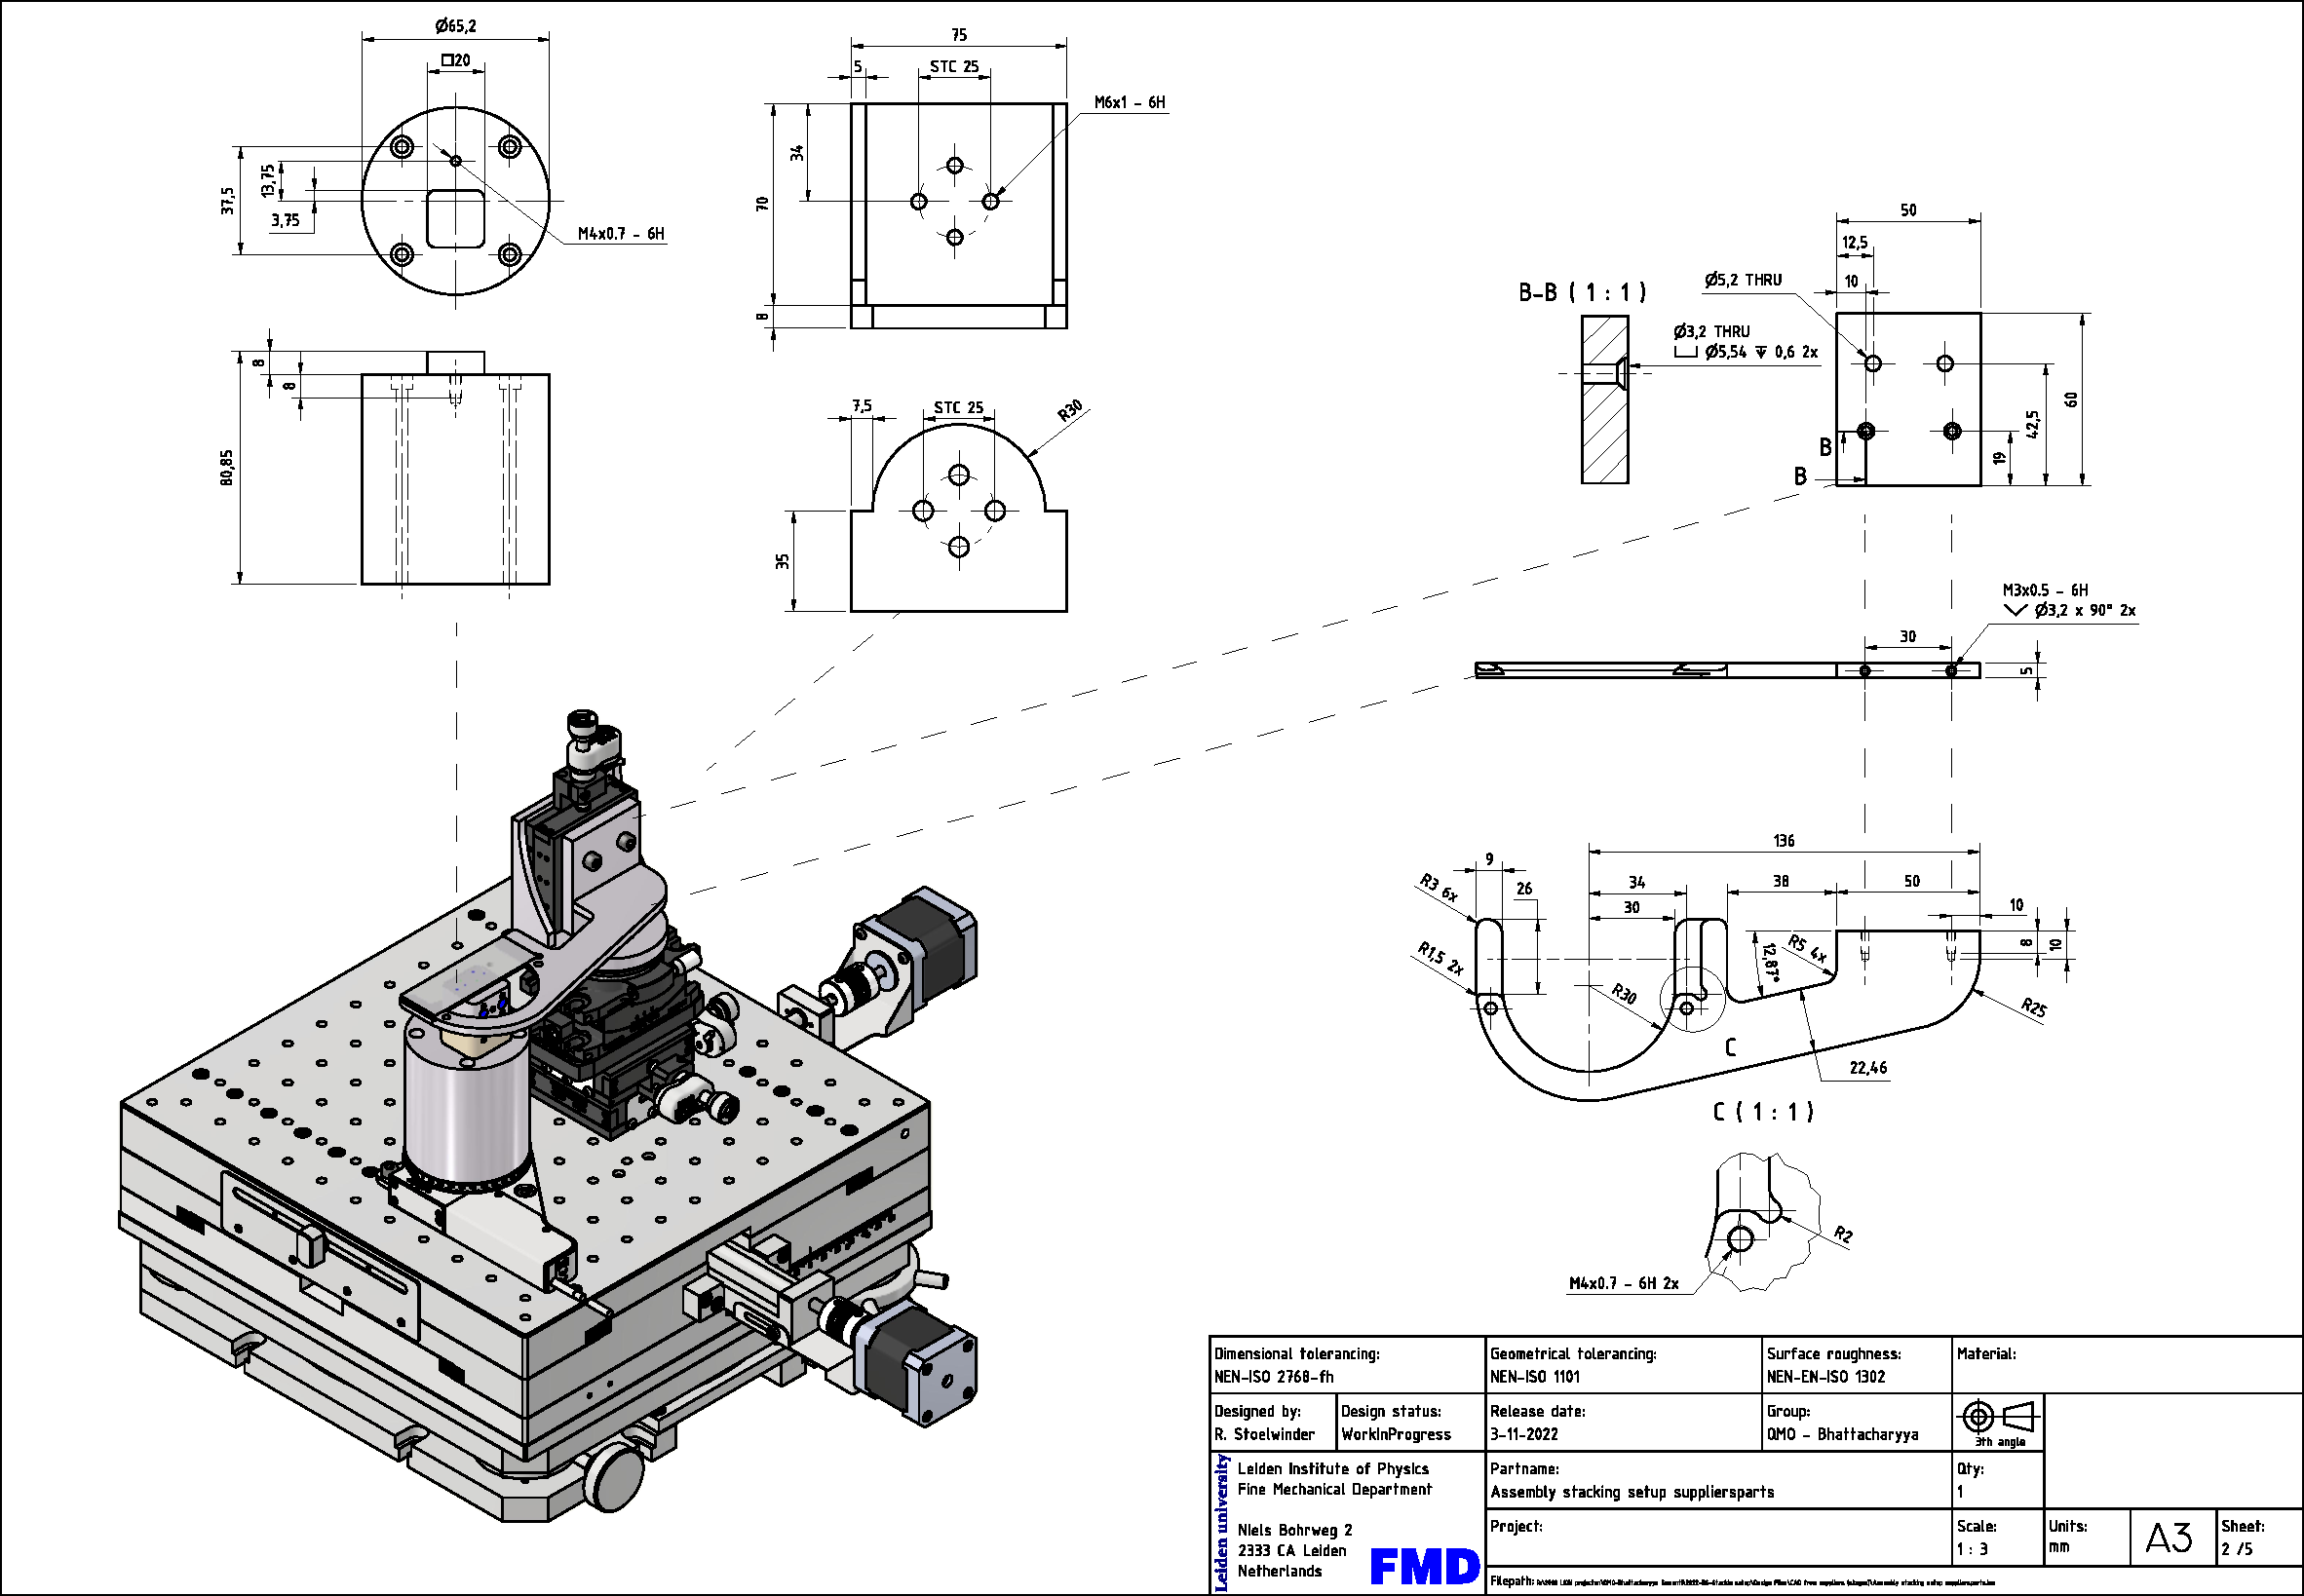
\includegraphics[angle=90,origin=c,width=\textwidth]{img/cad/pag2.pdf}
  \caption{Technical drawing of the used stages, mask and spacer bus. By R. Stoelwinder}
  \label{doc:tech_stages}
\end{figure}

\clearpage
\begin{figure}[htp]
  \centering
  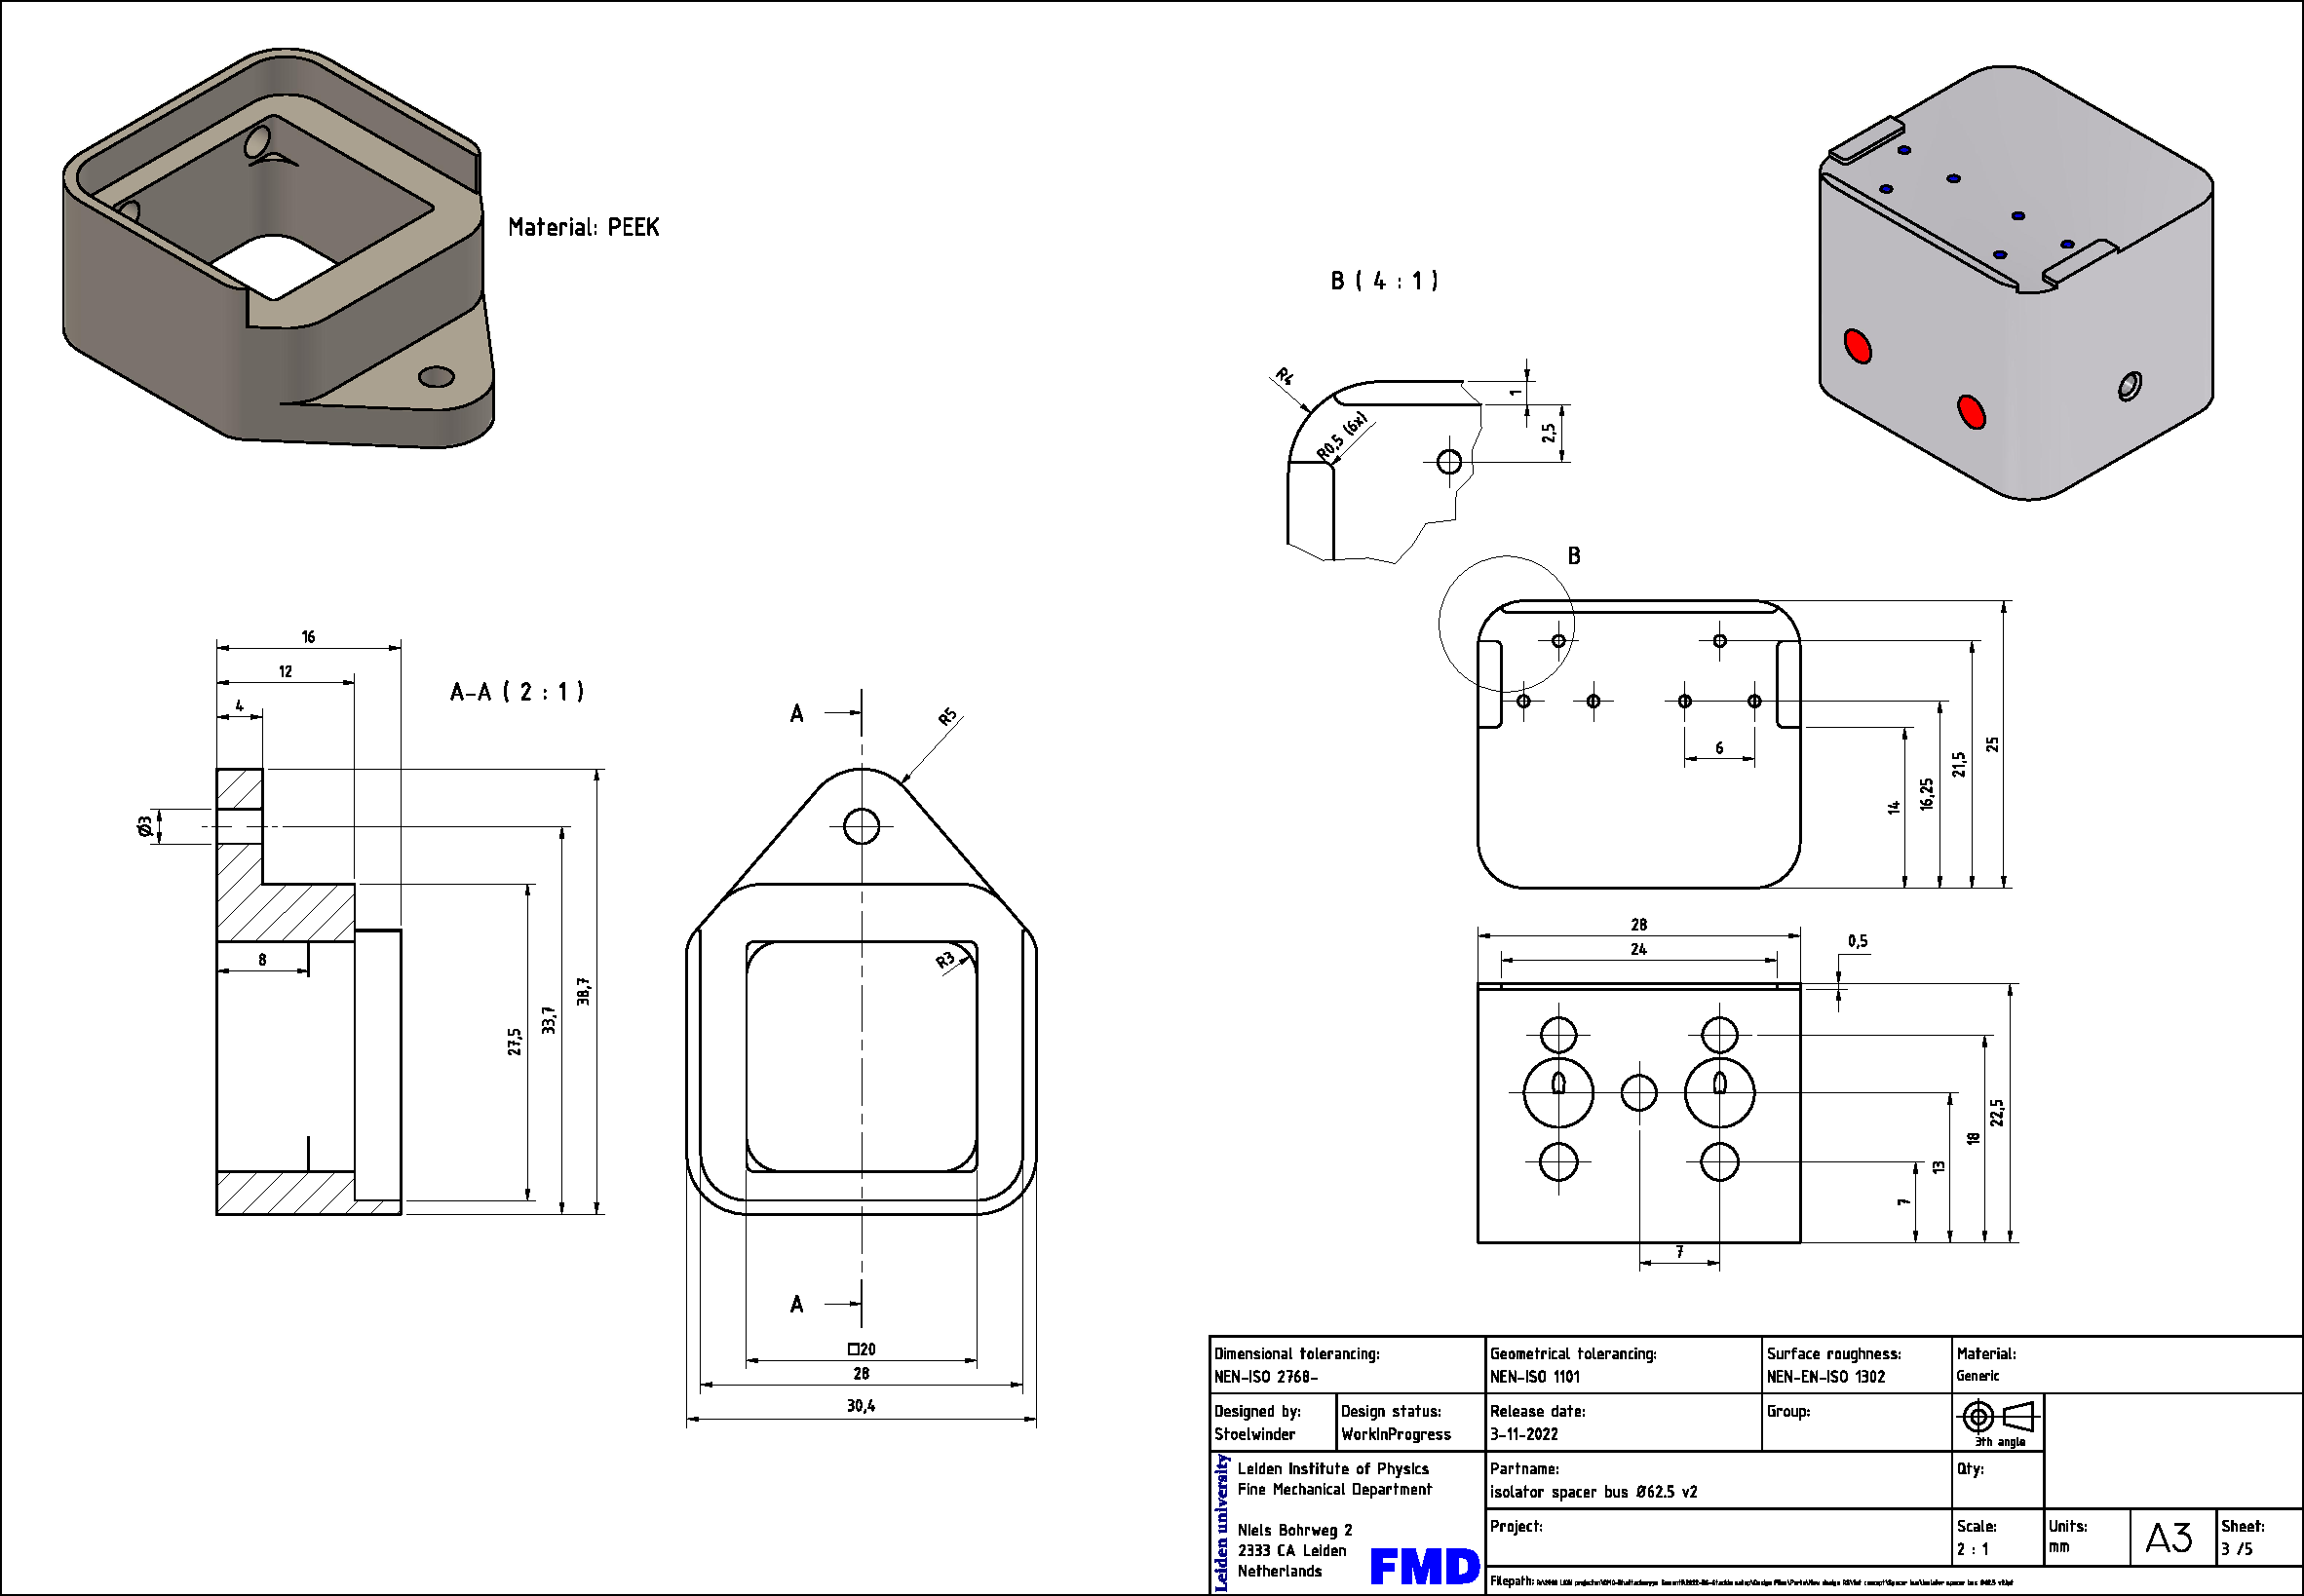
\includegraphics[angle=90,origin=c,width=\textwidth]{img/cad/pag3.pdf}
  \caption{Technical drawing of the sample bed ans used isolation shroud. By R. Stoelwinder}
  \label{doc:tech_bed}
\end{figure}

\clearpage
\begin{figure}[htp] 
  \centering
  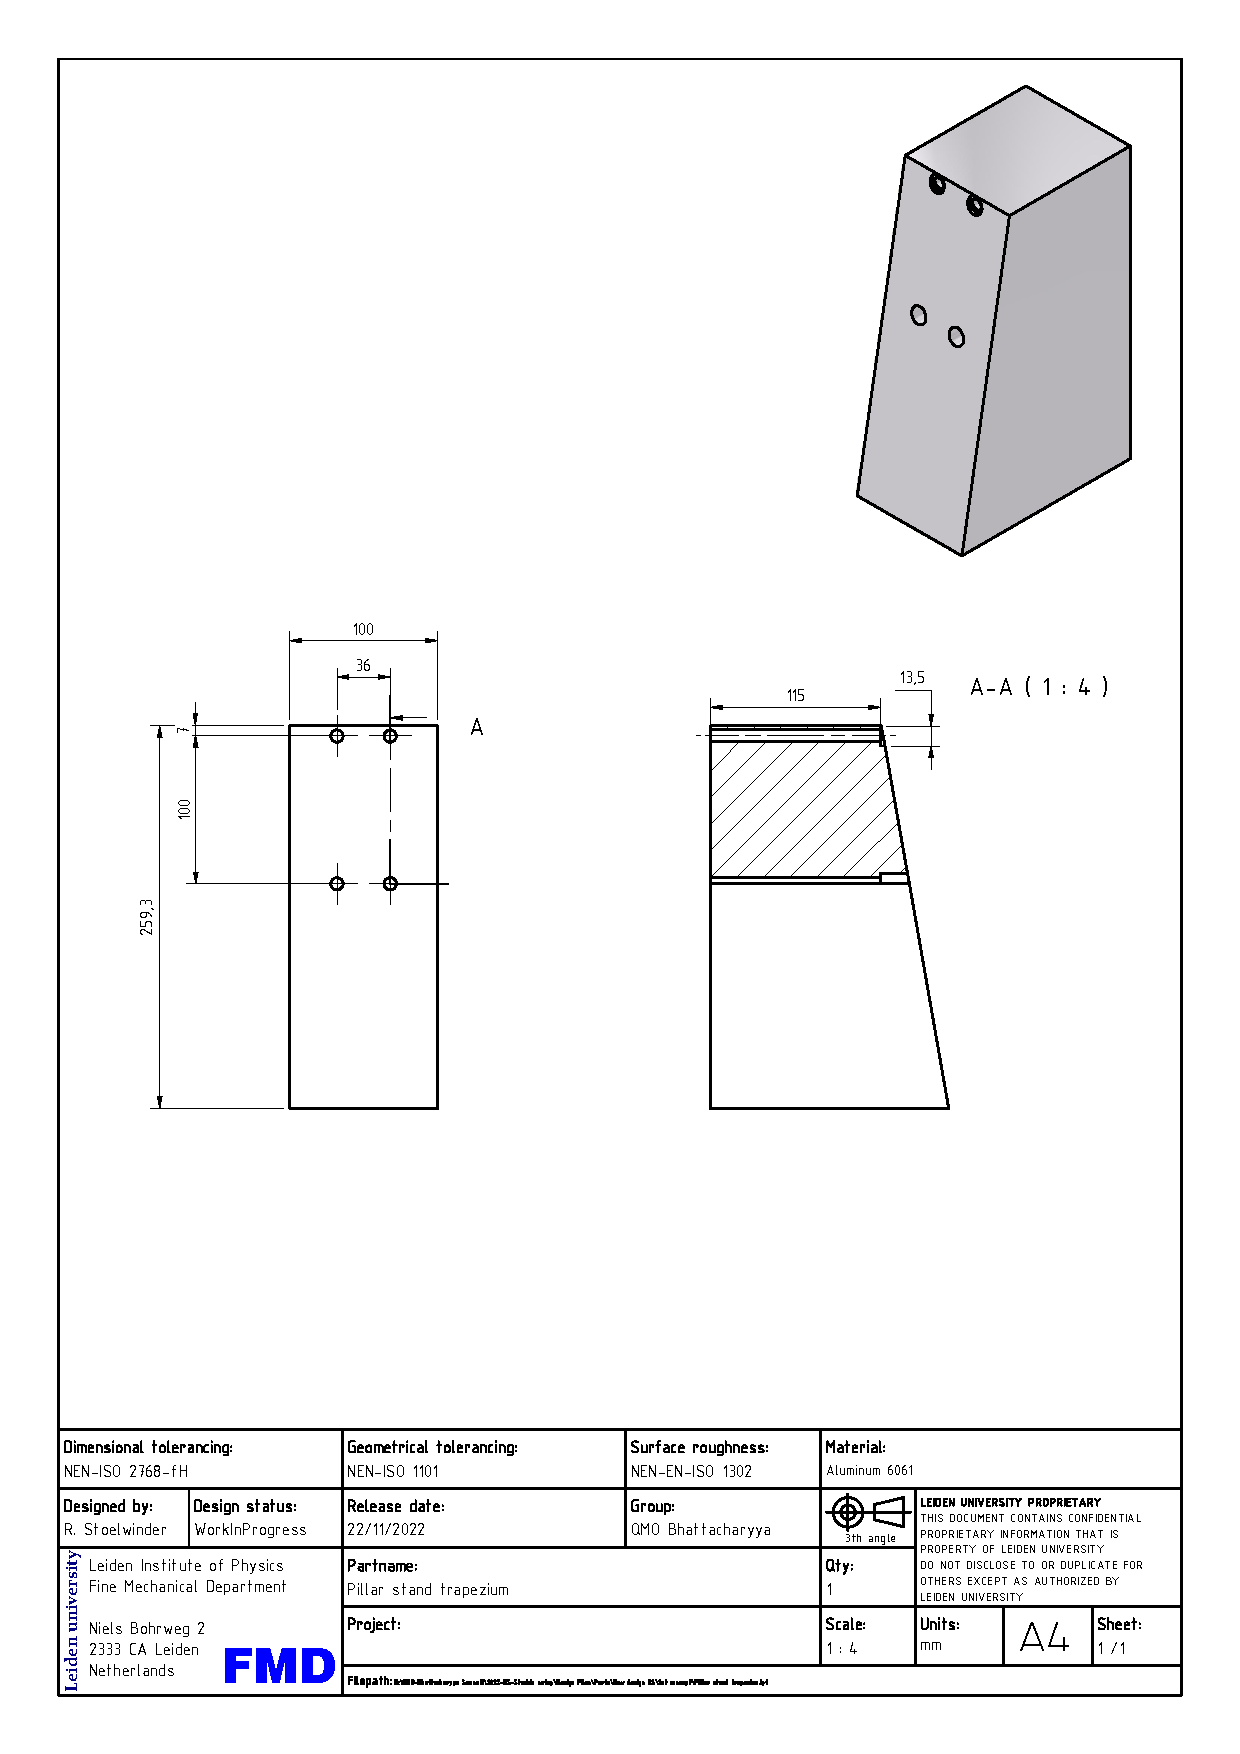
\includegraphics[origin=c,width=\textwidth]{img/cad/Pillar stand trapezium.0001.pdf}
  \caption{Technical drawing of the vertical stand mount. By R. Stoelwinder}
  \label{doc:tech_trap_mount}
\end{figure}

\clearpage
\begin{figure}[htp] 
  \centering
  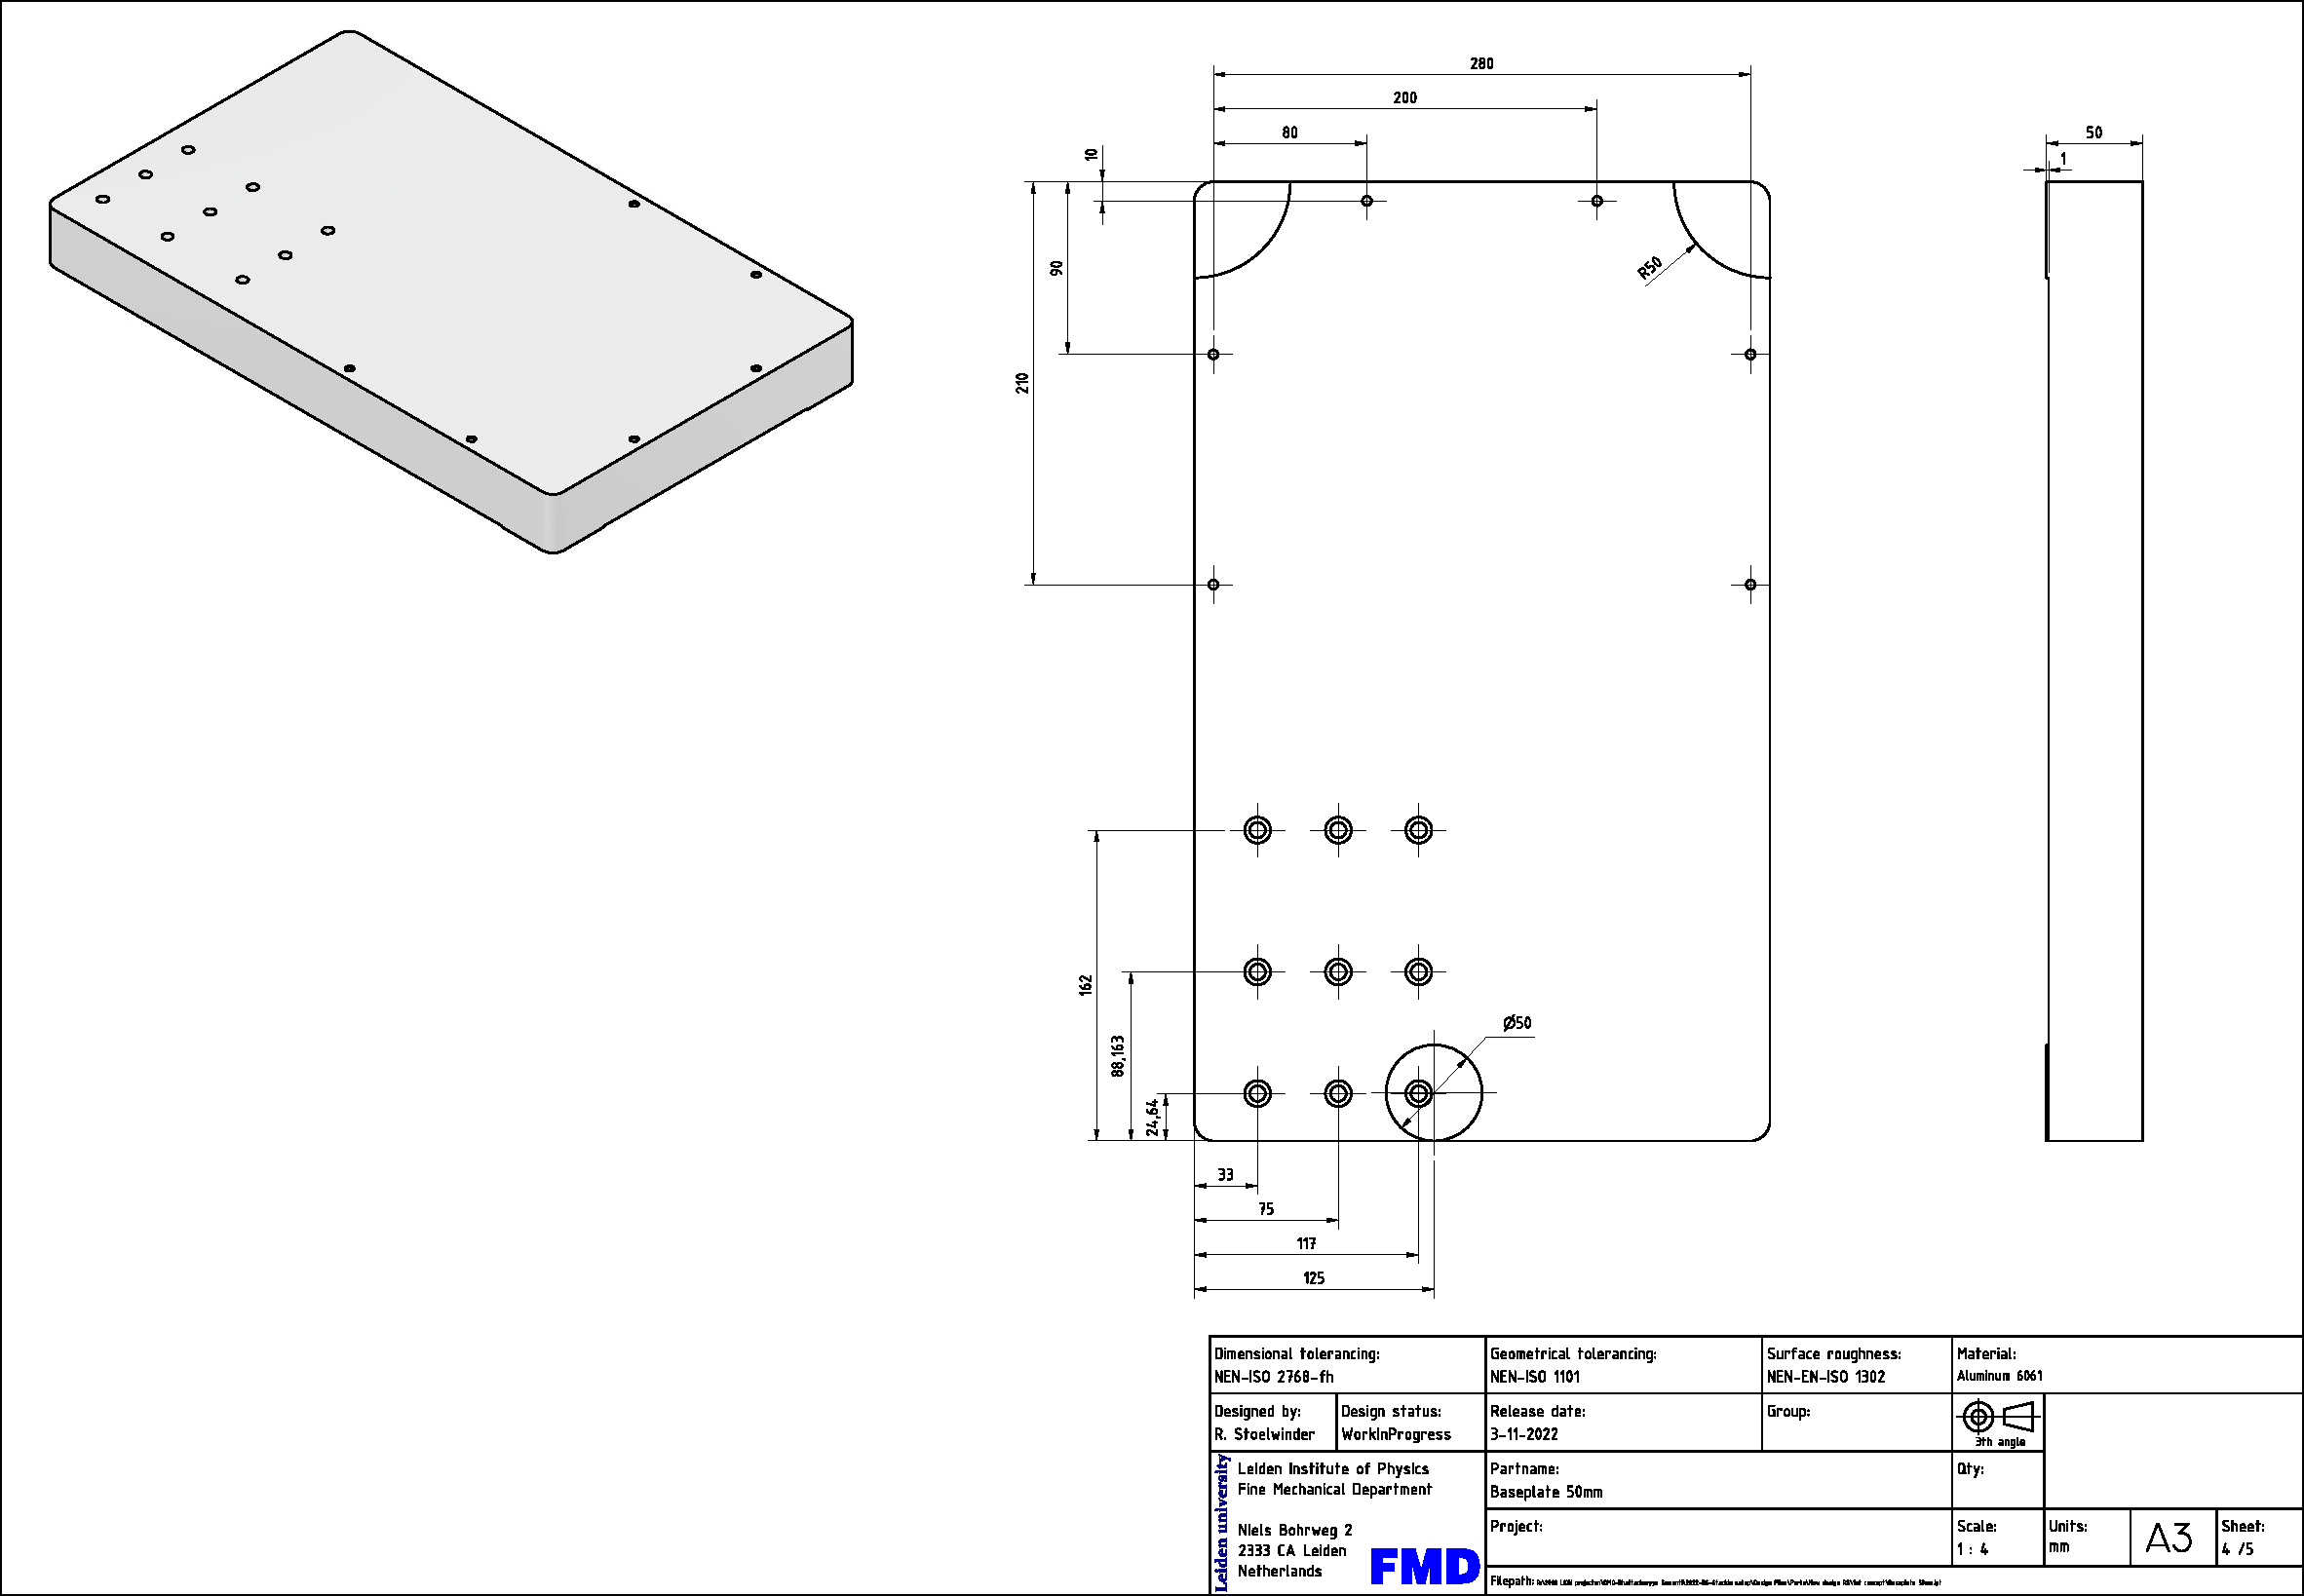
\includegraphics[angle=90,origin=c,width=\textwidth]{img/cad/pag4.pdf}
  \caption{Technical drawing of the stand base. By R. Stoelwinder}
  \label{doc:tech_base}
\end{figure}

\clearpage
\begin{figure}[htp] 
  \centering
  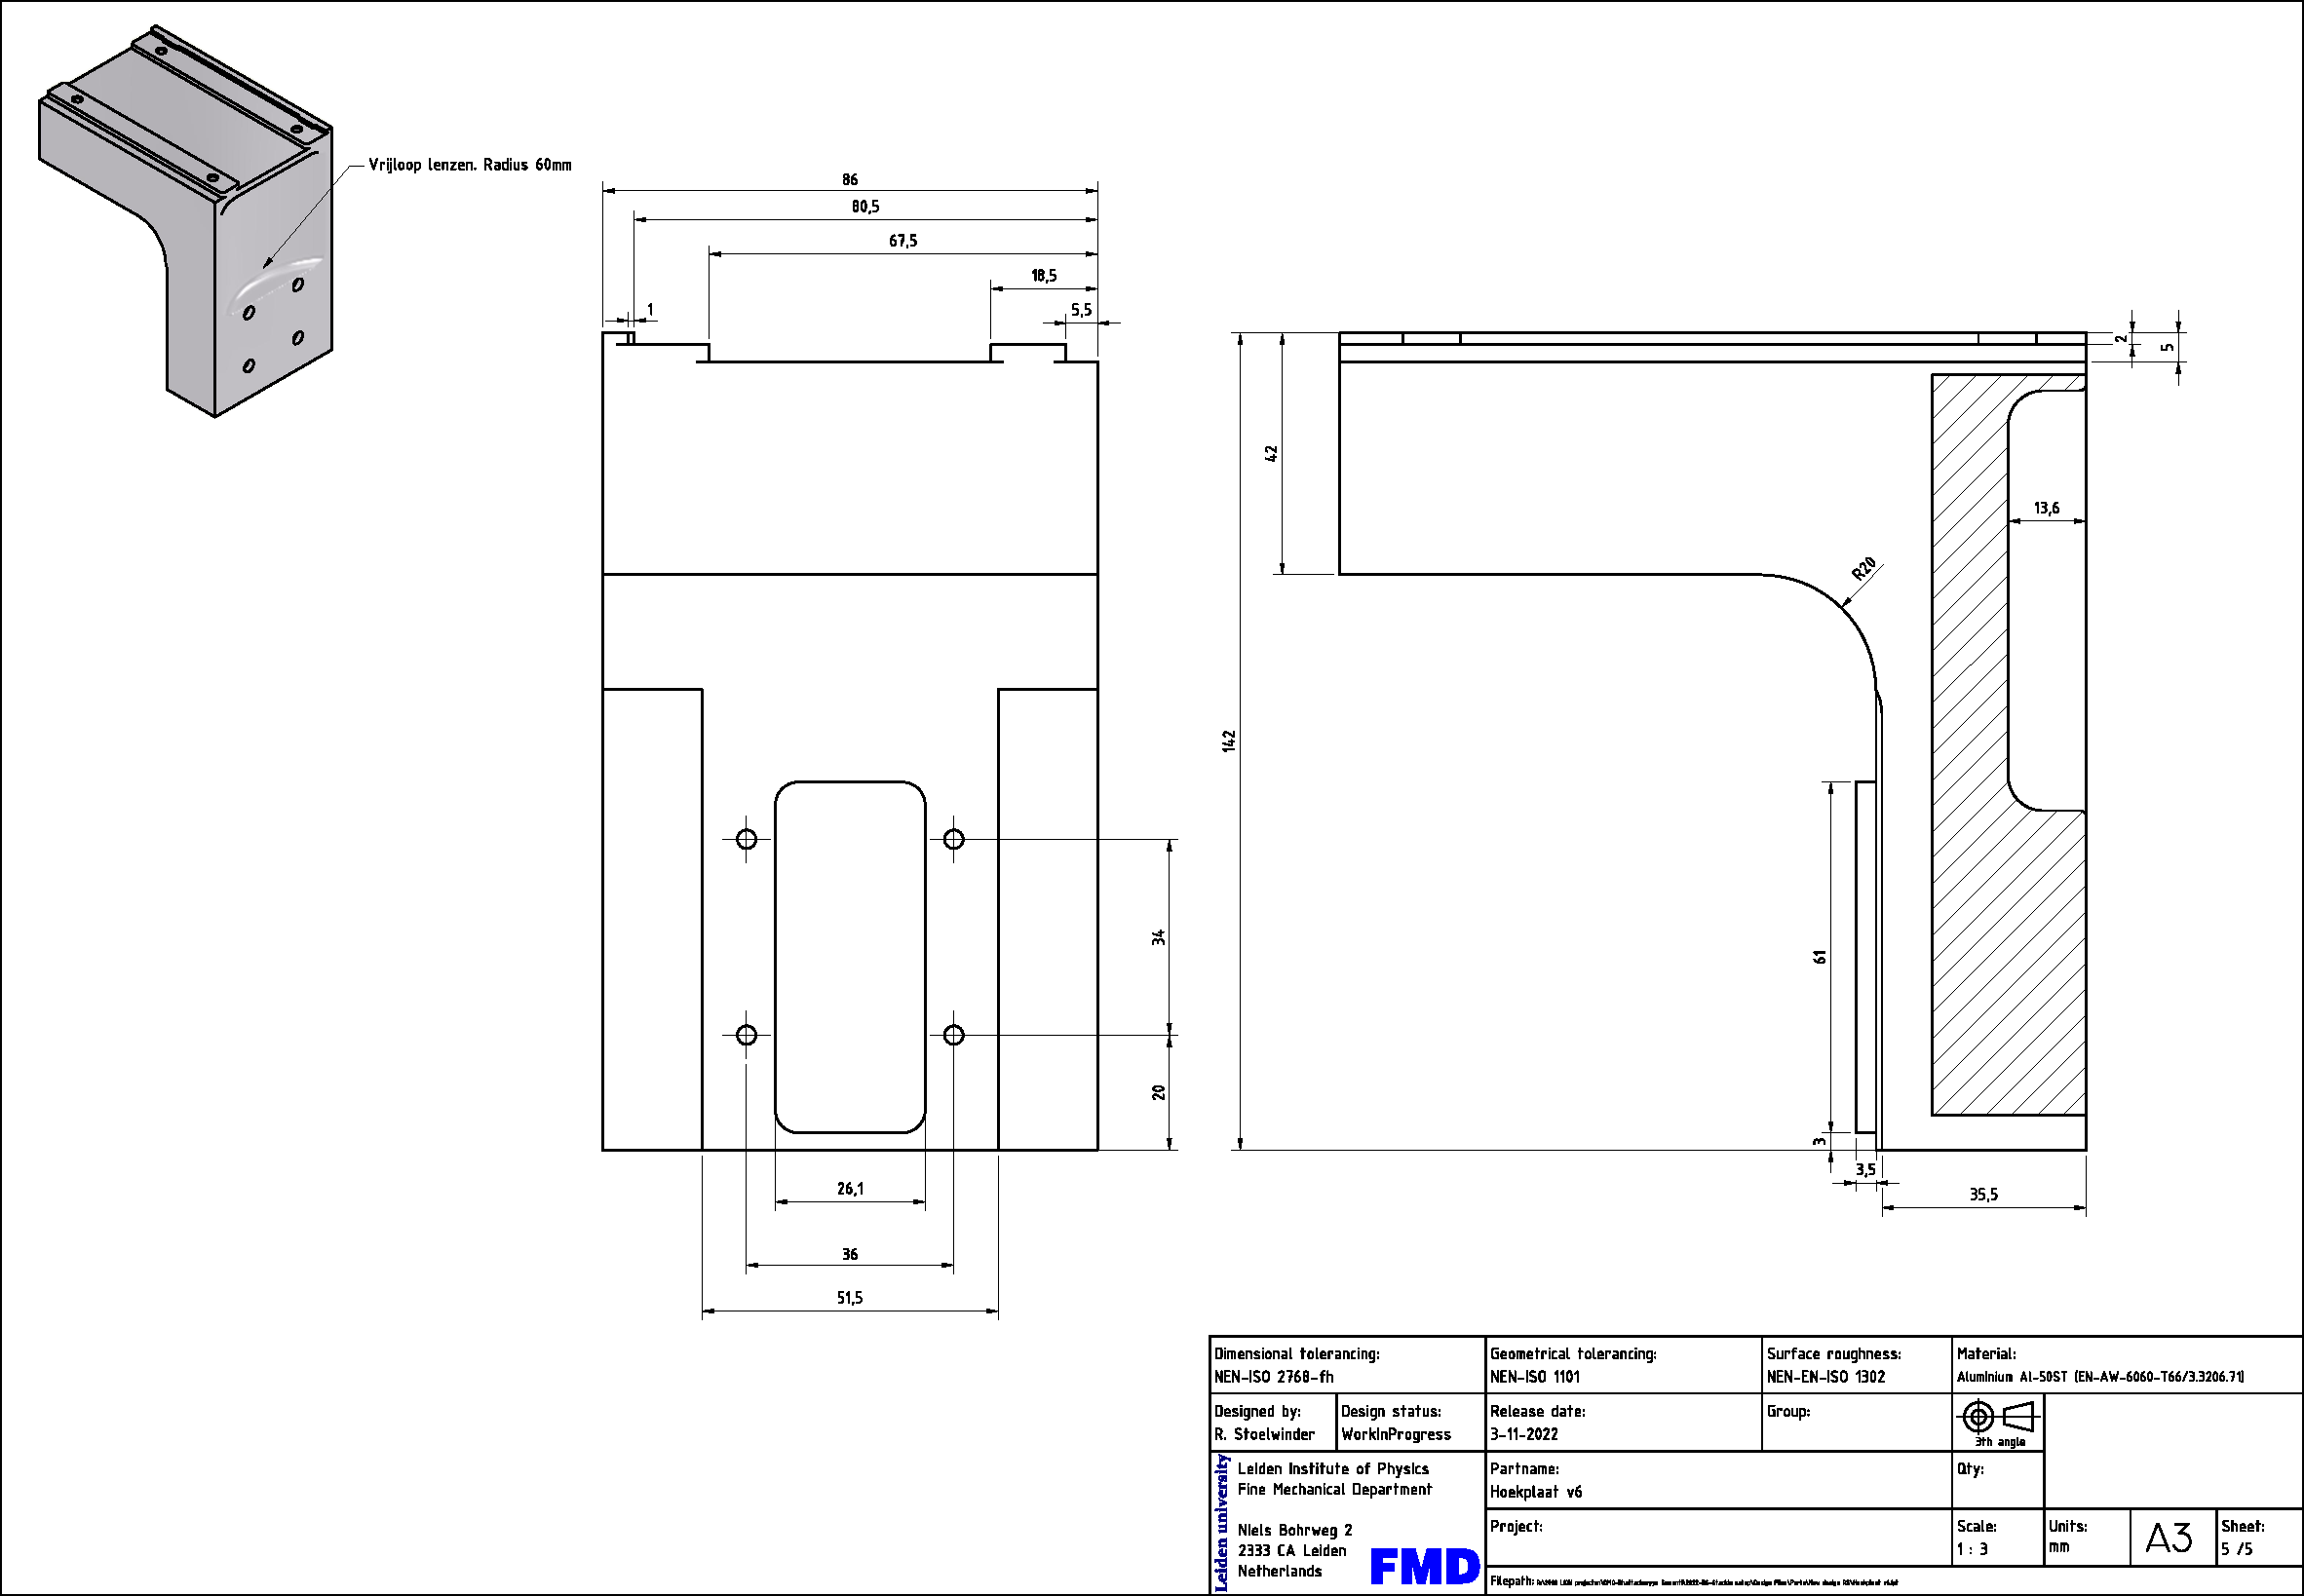
\includegraphics[angle=90,origin=c,width=\textwidth]{img/cad/pag5.pdf}
  \caption{Technical drawing of the microscope bracket. By R. Stoelwinder}
  \label{doc:tech_microscope_bracket}
\end{figure}




%\printbibliography

%\clearpage
%\section*{Appendix}



%\begin{figure}[H]
%  \centering
%  \begin{minipage}[b]{0.4\textwidth}
%    \includegraphics[width=\textwidth]{img/plot3.png}
%    \caption{ROC Curve: Random Plot 2}
%    \label{fig:Wrong_Orientation}
%  \end{minipage}
%  \hfill
%  \begin{minipage}[b]{0.4\textwidth}
%    \includegraphics[width=\textwidth]{img/plot4.png}
%    \caption{ROC Curve: Random Plot 2}
%    \label{fig:Unusual}
%  \end{minipage}
%\end{figure}

%****** Extra package work if needed
% To add math, use
%\begin{equation}
 %Helpful links    https://www.overleaf.com/learn/latex/Mathematical_expressions
%\end{equation}

%To add hyperlinks, use 
%For further references see \href{http://www.overleaf.com}{Something Linky} or go to the next url: \url{http://www.overleaf.com}

% It's also possible to link directly any word or \hyperlink{thesentence}{any sentence} in you document.

% Tables 

% \begin{table}[h!]
% \centering
%  \begin{tabular}{||c c c c||} 
%  \hline
%  Col1 & Col2 & Col2 & Col3 \\ [0.5ex] 
%  \hline\hline
%  1 & 6 & 87837 & 787 \\ 
%  2 & 7 & 78 & 5415 \\
%  3 & 545 & 778 & 7507 \\
%  4 & 545 & 18744 & 7560 \\
%  5 & 88 & 788 & 6344 \\ [1ex] 
%  \hline
%  \end{tabular}
% \end{table}

% Images

% upload your images to the img folder. To print them in the document, uncomment the following
% \begin{figure}[h]
%     \centering
%     \includegraphics[width=0.25\textwidth]{/img/YourImageTitle}
%     \caption{a nice plot}
%     \label{fig:mesh1}
% \end{figure}

% As you can see in the figure \ref{fig:mesh1}, the 
% function grows near 0. Also, in the page \pageref{fig:mesh1} 
% is the same example.

\clearpage
\todototoc
\listoftodos
\end{document}
